% Options for packages loaded elsewhere
\PassOptionsToPackage{unicode}{hyperref}
\PassOptionsToPackage{hyphens}{url}
\PassOptionsToPackage{dvipsnames,svgnames,x11names}{xcolor}
%
\documentclass[
  12pt,
]{article}
\usepackage{amsmath,amssymb}
\usepackage{lmodern}
\usepackage{iftex}
\ifPDFTeX
  \usepackage[T1]{fontenc}
  \usepackage[utf8]{inputenc}
  \usepackage{textcomp} % provide euro and other symbols
\else % if luatex or xetex
  \usepackage{unicode-math}
  \defaultfontfeatures{Scale=MatchLowercase}
  \defaultfontfeatures[\rmfamily]{Ligatures=TeX,Scale=1}
\fi
% Use upquote if available, for straight quotes in verbatim environments
\IfFileExists{upquote.sty}{\usepackage{upquote}}{}
\IfFileExists{microtype.sty}{% use microtype if available
  \usepackage[]{microtype}
  \UseMicrotypeSet[protrusion]{basicmath} % disable protrusion for tt fonts
}{}
\makeatletter
\@ifundefined{KOMAClassName}{% if non-KOMA class
  \IfFileExists{parskip.sty}{%
    \usepackage{parskip}
  }{% else
    \setlength{\parindent}{0pt}
    \setlength{\parskip}{6pt plus 2pt minus 1pt}}
}{% if KOMA class
  \KOMAoptions{parskip=half}}
\makeatother
\usepackage{xcolor}
\IfFileExists{xurl.sty}{\usepackage{xurl}}{} % add URL line breaks if available
\IfFileExists{bookmark.sty}{\usepackage{bookmark}}{\usepackage{hyperref}}
\hypersetup{
  pdftitle={Waterfowl Breeding Population Survey For Wisconsin, 1973--2022},
  colorlinks=true,
  linkcolor={blue},
  filecolor={Maroon},
  citecolor={Blue},
  urlcolor={blue},
  pdfcreator={LaTeX via pandoc}}
\urlstyle{same} % disable monospaced font for URLs
\usepackage[margin = 1in]{geometry}
\usepackage{graphicx}
\makeatletter
\def\maxwidth{\ifdim\Gin@nat@width>\linewidth\linewidth\else\Gin@nat@width\fi}
\def\maxheight{\ifdim\Gin@nat@height>\textheight\textheight\else\Gin@nat@height\fi}
\makeatother
% Scale images if necessary, so that they will not overflow the page
% margins by default, and it is still possible to overwrite the defaults
% using explicit options in \includegraphics[width, height, ...]{}
\setkeys{Gin}{width=\maxwidth,height=\maxheight,keepaspectratio}
% Set default figure placement to htbp
\makeatletter
\def\fps@figure{htbp}
\makeatother
\setlength{\emergencystretch}{3em} % prevent overfull lines
\providecommand{\tightlist}{%
  \setlength{\itemsep}{0pt}\setlength{\parskip}{0pt}}
\setcounter{secnumdepth}{5}
\newlength{\cslhangindent}
\setlength{\cslhangindent}{1.5em}
\newlength{\csllabelwidth}
\setlength{\csllabelwidth}{3em}
\newlength{\cslentryspacingunit} % times entry-spacing
\setlength{\cslentryspacingunit}{\parskip}
\newenvironment{CSLReferences}[2] % #1 hanging-ident, #2 entry spacing
 {% don't indent paragraphs
  \setlength{\parindent}{0pt}
  % turn on hanging indent if param 1 is 1
  \ifodd #1
  \let\oldpar\par
  \def\par{\hangindent=\cslhangindent\oldpar}
  \fi
  % set entry spacing
  \setlength{\parskip}{#2\cslentryspacingunit}
 }%
 {}
\usepackage{calc}
\newcommand{\CSLBlock}[1]{#1\hfill\break}
\newcommand{\CSLLeftMargin}[1]{\parbox[t]{\csllabelwidth}{#1}}
\newcommand{\CSLRightInline}[1]{\parbox[t]{\linewidth - \csllabelwidth}{#1}\break}
\newcommand{\CSLIndent}[1]{\hspace{\cslhangindent}#1}
\usepackage{booktabs}
\usepackage{colortbl}
\usepackage{tabu}
\usepackage{threeparttable}
\usepackage{makecell}
\renewcommand{\contentsname}{Table of Contents}
\ifLuaTeX
  \usepackage{selnolig}  % disable illegal ligatures
\fi

\title{Waterfowl Breeding Population Survey For Wisconsin, 1973--2022}
\author{Jason Winiarski\textsuperscript{1} and Taylor
Finger\textsuperscript{2}\\
\emph{\textsuperscript{1}Office of Applied Science}\\
\emph{\textsuperscript{2}Bureau of Wildlife Management}\\
\emph{Wisconsin Department of Natural Resources}}
\date{April 2023}

\begin{document}
\maketitle

{
\hypersetup{linkcolor=}
\setcounter{tocdepth}{3}
\tableofcontents
}
\newpage

\hypertarget{abstract}{%
\section{Abstract}\label{abstract}}

The 2022 Waterfowl Breeding Population Survey for Wisconsin was
conducted from April 25--May 6 and followed methods of the North
American Waterfowl Breeding Population and Habitat Survey. The
information from this survey is used as part of the overall survey of
breeding waterfowl in North America as well as in making state-level
waterfowl management decisions. This survey has been conducted annually
since 1973, and data on Wisconsin waterfowl breeding populations and
wetland counts are best interpreted as trends over several years rather
than as year-to-year fluctuations.

Total non-linear basins were up 87.1\% from 2021 in the Southeast
Central (SEC) region and up 116.2\% from the long-term, 49-year mean. In
the Northern High Density (NHI) region, total non-linear basins were up
70.1\% from 2021 and up 105.9\% from the long-term mean. Non-linear
basins were up 149.7\% from 2021 in the Northern Low Density (NLO)
region and up 224.5\% from the long-term mean. Non-linear basins were up
40.1\% from 2021 in the Southwest Driftless (SWD) region and up 32.9\%
compared to this region's long-term (25-year) mean. Total linear basins
were up 25.8\% from 2021 in the SEC region and up 58.6\% from the
long-term mean. In the NHI region, linear basins were up 73.5\% from
2021 and up 120.3\% from the long-term mean. NLO region linear basins
were up 47.1\% from 2021 and up 108.0\% from the long-term mean. Linear
basins were down 16.2\% from 2021 in the SWD region and up 16.4\% from
the long-term mean.

The 2022 total breeding duck modeled population estimate of 591,762 was
6.3\% higher than the 2021 modeled estimate of 556,507, and was 33.6\%
higher than the long-term mean. Overall, the total duck population
estimate for 2022 was higher than what we have experienced over the last
few years (2015--2019) and above the total duck numbers experienced in
the prior 10 years. The mallard modeled breeding population estimate of
181,686 was 3.3\% higher than the 2021 estimate of 175,819 and was 1.5\%
higher than the long-term mean. The blue-winged teal modeled breeding
population estimate of 81,359 was 9.0\% higher compared to the 2021
estimate of 74,653, but remains 22.1\% lower than the long-term mean. At
174,526 the 2022 population estimate for wood ducks was 8.4\% lower than
the 2021 estimate of 190,551 and 102.2\% higher than the long-term mean.
The modeled Canada goose population estimate of 180,340 was 3.3\% higher
compared to the 2021 estimate of 174,515, and 68.2\% higher than the
long-term mean. The population estimate of ``other ducks'' was 156,330,
which was 26.4\% higher than the 2021 estimate of 123,648 and was
138.8\% higher than the long-term mean.

\newpage

\hypertarget{introduction}{%
\section{Introduction}\label{introduction}}

Decisions regarding hunting season structure and harvest limits in
waterfowl management are based in part upon spring breeding pair
surveys. The U.S. Fish and Wildlife Service's (USFWS)
\href{https://www.fws.gov/project/waterfowl-breeding-population-and-habitat-survey}{Waterfowl
Breeding Population and Habitat Survey (BPOP)} has been conducted for 68
years across the traditional survey area of the north-central United
States, Canada and Alaska. The Wisconsin Waterfowl Breeding Population
Survey--which is modeled after the BPOP--has been conducted since 1973
and provides a long-term record of waterfowl breeding trends and wetland
counts in Wisconsin. These data are used at the national- and
state-level for monitoring waterfowl populations and making management
decisions. Wisconsin's breeding waterfowl survey data are included in
the
\href{https://www.fws.gov/sites/default/files/documents/WaterfowlPopulationStatusReport21.pdf}{Waterfowl
Population Status report} published annually by the USFWS on continental
waterfowl populations. In addition, mallard data from Wisconsin,
Minnesota, and Michigan are combined with data from the traditional
survey area as a basis for the USFWS's
\href{https://www.fws.gov/sites/default/files/documents/adaptive-harvest-management-hunting-season-report-2022.pdf}{Adaptive
Harvest Management report} that is used to establish federal waterfowl
season frameworks. At the state-level, waterfowl breeding survey data
are used to inform annual hunting season regulations, identify long-term
changes in population trends, and evaluate the impacts of habitat
changes and management. This report provides a summary and analysis of
the 2022 survey data in support of these efforts.

\hypertarget{methods}{%
\section{Methods}\label{methods}}

\hypertarget{study-area-and-survey-timing}{%
\subsection{Study area and survey
timing}\label{study-area-and-survey-timing}}

The Wisconsin Waterfowl Breeding Population Survey employs a stratified
sampling scheme modeled after the BPOP survey (Platte 1987) but modified
for local conditions (March et al. 1973). The state is divided into four
strata based on regional waterfowl densities and habitat attributes: the
Southeast Central region (SEC), Northern High Density region (NHI),
Northern Low Density region (NLO), and Southwest Driftless region (SWD;
Figure \ref{fig:transect_map}). Fifty-five east-west oriented transects,
each 30 mi in length and 1/4 mi-wide, were randomly selected in 1973
within the SEC (\emph{n} = 29), NHI (\emph{n} = 13), and NLO (\emph{n} =
13) regions; transects in the SWD region (\emph{n} = 11) were not added
until 1997 due to low wetland density. Surveys have been conducted every
year since 1973, except in 2020 due to the COVID-19 pandemic.

Transects are typically surveyed from May 1--20 to obtain accurate
estimates of \emph{local} breeding pairs. However, the start date may be
adjusted to accommodate inter-annual variation in the timing of spring
(i.e., to exclude migratory individuals and minimize the effects of
leaf-out on observer visibility). To account for latitudinal differences
in leaf-out and waterfowl breeding phenology, surveys are generally
initiated in southern Wisconsin and northern transects are the last to
be completed.

\hypertarget{data-collection}{%
\subsection{Data collection}\label{data-collection}}

Two observers--each experienced in waterfowl identification and
waterfowl census procedures--performed the aerial surveys. To minimize
problems with observer bias, the same aerial observers are used for a
minimum five-year period. In addition, surveys do not take place when
winds exceed 25 mph or if other adverse weather conditions exist (e.g.,
snow, rain, fog, and smoke). Fixed-wing aerial surveys were conducted
from a Cessna 182 aircraft, flying at 90--100 mph and 100--150 ft above
ground level. During each transect flight, an observer recorded all
observations of ducks, geese, coots, cranes, and swans within a 1/8-mile
strip from either side of the aircraft, while the observer on the north
side of the plane recorded the number and type of unoccupied wetland
basins containing surface water. All wetlands within the 1/4-mile
transect width on which breeding waterfowl are observed (i.e., occupied
wetlands) are also recorded by the observer counting waterfowl.

Given the challenges of detecting and counting waterfowl from the air,
27 segments of selected aerial transects are censused by ground crews to
obtain a `complete' count of all waterfowl present and calculate
visibility (air-to-ground) correction factors (VCFs). Ground crews (2--4
individuals) cover every wetland basin within a transect segment on foot
or by boat on the same day or within 2 days after the air count. Ground
observers record waterfowl observations according to the same
instructions for the aerial survey.

\hypertarget{data-preparation}{%
\subsection{Data preparation}\label{data-preparation}}

The Waterfowl Breeding Population Survey focuses on four priority
waterfowl species: mallards (\emph{Anas platyrhynchos}), blue-winged
teal (\emph{A. discors}), wood ducks (\emph{Aix sponsa}) and Canada
geese (\emph{Branta canadensis}). All other duck species that are likely
breeders in Wisconsin are pooled into a category of ``other ducks''
(``total ducks'' combines these four priority species and ``other
ducks''). By 2004, wood duck populations had increased to a level where
we were able to estimate them as a separate group rather than as part of
``other ducks.'' Lesser scaup (\emph{Aythya affinis}) and bufflehead
(\emph{Bucephala albeola}) are not included in population estimates
because they rarely breed in Wisconsin and when counted are assumed to
be in migration to more northern breeding areas. We also tallied counts
for several other species of interest: American coots (\emph{Fulica
americana}), whooping cranes (\emph{Grus americana}), sandhill cranes
(\emph{Antigone canadensis}), and trumpeter swans (\emph{Cygnus
buccinator}).

We note that this survey was not originally designed for surveying
Wisconsin's resident Canada goose population due to their earlier
breeding phenology. However, aerial counts of geese increased steadily
from the mid-1980s through the early 2000s, making survey estimates
useful indices of population trends. Human-goose conflicts resulting
from a growing goose population increase the importance of tracking the
population status of breeding geese in Wisconsin, and have been included
in this report since 1986.

Prior to analysis, we calculated the total numbers of ``indicated''
birds for each transect based on the observation type (i.e., pairs, lone
drakes, flocked drakes {[}males in groups of 2--4{]}, and groups
{[}\(\geq\) 5 drakes or mixed flocks that cannot be separated into pairs
or sexes{]}) and each species' breeding biology. In general, lone
drakes, flocked drakes, and pairs are adjusted by a multiplier of two,
while groups are not adjusted.

\hypertarget{statistical-analysis}{%
\subsection{Statistical analysis}\label{statistical-analysis}}

\hypertarget{visibility-correction-factors}{%
\subsubsection{Visibility correction
factors}\label{visibility-correction-factors}}

The VCF (also referred to as \emph{R}; see below) is the ratio of
individuals counted by ground crews to the number of individuals counted
by aerial crews from the same set of transect segments. VCFs are used as
a multiplier to the aerial survey counts and yield statewide, corrected
abundance estimates. VCFs were calculated independently for all priority
waterfowl species and ``other ducks'' by pooling data from all 27
air/ground transect segments. To quantify VCF precision, we calculated
the coefficient of variation (CV), which provides a standardized measure
of dispersion. We iteratively added prior years of survey data until a
CV value \(\leq\) 0.20 (and a robust VCF) was achieved.

\hypertarget{population-estimates}{%
\subsubsection{Population estimates}\label{population-estimates}}

To calculate species-specific and visibility-corrected abundance
estimates in each region, we used the traditional formula developed by
Smith (1995):

\begin{equation}
{\text{\textit{N}}} = {\text{\textit{B}}} \times {\text{\textit{A}}} \times {\text{\textit{R}}}
\end{equation}

where \emph{B} is the bird density per mi\textsuperscript{2}, \emph{A}
is the area of the survey region, and \emph{R} is the visibility
correction factor. We note that this procedure was only conducted for
the four priority waterfowl species and ``other ducks'' (VCF-corrected
estimates were summed across these groups to estimate ``total duck''
abundance).

Because these abundance estimates are imperfect counts (i.e., some
combination of true population size and detection error), we elected to
model annual trends using a Bayesian state-space modeling approach (Kéry
and Schaub 2012). State-space models are hierarchical models that
simultaneously account for process error (true population size change)
and measurement error (survey biases), and are increasingly used to
model ecological time series (Auger-Méthé et al. 2021). State-space
models offer at least two important advantages. First, modeled survey
estimates smooth out drastic annual changes in population estimates that
are biologically unrealistic (e.g., mallard abundance changing from
roughly 250,000 in 1999, 450,000 in 2000, and then 180,000 in 2001).
Second, a Bayesian state-space model allows for prediction, even when
counts are unavailable (e.g., when surveys were canceled in 2020 due to
the COVID-19 pandemic). Therefore, in the following waterfowl summaries
we reference abundance and percent changes in state-space estimates
rather than the raw population estimates. However, for comparison and
continuity with previous reports, we provide both estimate types in the
associated tables and figures (state-space modeling was first
implemented for the 2021 report). We report the mean population estimate
and 95\% credible interval (CI), which can be interpreted as saying
`\emph{the true population size has a 95\% probability of falling within
this range, given the observed data}.'

\hypertarget{results}{%
\section{Results}\label{results}}

\hypertarget{survey-timing}{%
\subsection{Survey timing}\label{survey-timing}}

We initiated the 2022 Waterfowl Breeding Population Survey on April 25.
As in the past, the survey was initiated in the southern part of
Wisconsin, progressing northward to account for the differences in
phenology from south to north. The timing of the breeding waterfowl
survey is always a challenge because variables such as weather,
waterfowl phenology, and tree leaf-out all impact the timing, visibility
and accuracy of the survey. Weather was a slight issue leading up to and
during the survey, with extremely wet conditions across most of the
state and cold conditions in the north, resulting in northern Wisconsin
lakes retaining some ice into late April/early May. Significant rainfall
events likely contributed to the high number of temporary and other
wetland types recorded across much of the state.

Aerial surveys were completed in 9 days from April 25 to May 5. The
ground survey was completed in 10 days from April 26 to May 6. Paired
aerial and ground surveys occurred within 2 days of each other, except
for one transect segment where aerial/ground surveys occurred within 3
days.

\hypertarget{wetland-counts}{%
\subsection{Wetland counts}\label{wetland-counts}}

In the SEC region, total non-linear basins were up 87.1\% from 2021 and
were up 116.2\% from the long-term (49-year) mean. Linear basins in the
SEC region were up 25.8\% from 2021 and up 58.6\% from the long-term
mean (Table \ref{tab:wetland_tab_sec}). In the NHI region, total
non-linear basins were up 70.1\% from 2021 and up 105.9\% from the
long-term mean. Linear basins in the NHI region were up 73.5\% from 2021
and up 120.3\% from the long-term mean (Table
\ref{tab:wetland_tab_nhi}). In the NLO region, total non-linear basins
were up 149.7\% from 2021 and up 224.5\% from the long-term mean. Linear
basins in the NLO region were up 47.1\% from 2021 and up 108.0\% from
the long-term mean (Table \ref{tab:wetland_tab_nlo}). In the SWD region,
total non-linear basins were up 40.1\% from 2021 and up 32.9\% from this
region's long-term, 25-year mean. Linear basins in the SWD region were
down 16.2\% from 2021 and up 16.4\% from the long-term mean (Table
\ref{tab:wetland_tab_swd}). Long-term wetland counts for each survey
region are shown in Figure \ref{fig:wetland_abundance}.

\hypertarget{waterfowl-population-estimates}{%
\subsection{Waterfowl population
estimates}\label{waterfowl-population-estimates}}

2022 VCF and population estimate summary statistics for mallards,
blue-winged teal, wood ducks, ``other ducks'', and Canada geese are
provided in Table \ref{tab:current_breeding_estimate_table}.

\hypertarget{mallards}{%
\subsubsection{Mallards}\label{mallards}}

The 2022 modeled mallard population estimate was \textbf{181,686 (95\%
credible interval {[}CI{]} = 136,200--237,762 individuals)}. This
estimate is 3.3\% higher compared to the previous year's modeled
estimate and 1.5\% higher than the long-term, 49-year mean (Table
\ref{tab:annual_state_space_estimates_table}; Figure
\ref{fig:ssm_mall}). As in previous years, the SEC still represented the
largest portion of the breeding mallard population (46\%) and was
similar to that of 2021.

\hypertarget{blue-winged-teal}{%
\subsubsection{Blue-winged teal}\label{blue-winged-teal}}

The 2022 modeled population estimate for blue-winged teal was
\textbf{81,359 (95\% CI = 48,810--129,071 individuals)}. This estimate
was 9.0\% higher compared to the previous year's modeled estimate but
remains 22.1\% lower than the long-term mean (Table
\ref{tab:annual_state_space_estimates_table}; Figure
\ref{fig:ssm_bwte}).

\hypertarget{wood-ducks}{%
\subsubsection{Wood ducks}\label{wood-ducks}}

The 2022 population estimate for wood ducks was \textbf{174,526 (95\% CI
= 111,751--262,979 individuals)}. This estimate was 8.4\% lower compared
to the previous year and was 102.2\% higher than the long-term mean
(Table \ref{tab:annual_state_space_estimates_table}; Figure
\ref{fig:ssm_wodu}). The breeding wood duck population showed
significant gains in the 1980s and early 1990s and appears to be
leveling off around 100,000 after peaking about 10 years ago but has
shown an increasing trend over the past five years.

\hypertarget{other-ducks}{%
\subsubsection{Other ducks}\label{other-ducks}}

The 2022 modeled population estimate for ``other ducks'' was
\textbf{156,330 (95\% CI = 73,792--285,474 individuals)}. This estimate
was 26.4\% higher compared to the previous year and was 138.8\% higher
than the long-term mean (Table
\ref{tab:annual_state_space_estimates_table}; Figure
\ref{fig:ssm_other_ducks}). Species considered as ``other ducks'' and
their percent composition in the 2022 uncorrected aerial count were:
American black duck (\emph{A. rubripes}; 0\%), northern pintail
(\emph{A. acuta}; 3\%), gadwall (\emph{Mareca strepera}; 0\%), American
wigeon (\emph{M. americana}; 0\%), northern shoveler (\emph{Spatula
clypeata}; 10\%), green-winged teal (\emph{A. carolinensis}; 4\%),
canvasback (\emph{A. valisineria}; 2\%), redhead (\emph{A. americana};
0\%), ring-necked duck (\emph{A. collaris}; 36\%), common goldeneye
(\emph{B. clangula}; 10\%), hooded merganser (\emph{Lophodytes
cucullatus}; 7\%), common merganser (\emph{Mergus merganser}; 24\%),
red-breasted merganser (\emph{M. serrator}; 0\%), and ruddy duck
(\emph{Oxyura jamaicensis}; 3\%).

\hypertarget{total-ducks}{%
\subsubsection{Total ducks}\label{total-ducks}}

The 2022 population estimate for all breeding ducks was \textbf{591,762
(95\% CI = 440,343--767,764 individuals)}. This estimate was 6.3\%
higher compared to the previous year and is 33.6\% higher than the
long-term mean (Table \ref{tab:annual_state_space_estimates_table};
Figure \ref{fig:ssm_total_ducks}).

\hypertarget{canada-geese}{%
\subsubsection{Canada geese}\label{canada-geese}}

Based on the most recent harvest derivations, the proportion of the
Wisconsin Canada goose harvest that consists of temperate breeding
(formerly `giant') Canada geese is about 60\%, with most of those birds
representing Canada geese that breed in Wisconsin (Dooley 2017). This
proportion indicates the continued importance of in-state breeding
Canada geese in our overall fall harvest. The 2022 population estimate
for Canada geese was \textbf{180,340 (95\% CI = 132,921--245,447
individuals)}. This estimate was 3.3\% higher than the previous year's
modeled estimate and was 68.2\% higher than the long-term, 36-year mean
(Table \ref{tab:annual_state_space_estimates_table}; Figure
\ref{fig:ssm_cago}). The long-term trend in goose numbers suggests a
continued, gradual increase in their population.

\hypertarget{american-coots-sandhill-cranes-and-trumpeter-swans}{%
\subsubsection{American coots, sandhill cranes, and trumpeter
swans}\label{american-coots-sandhill-cranes-and-trumpeter-swans}}

In 2022, observers counted a total of 422 coots, one pair of whooping
cranes, and 80 sandhill cranes (Figure \ref{fig:annual_crane_counts}).
Excluding groups of five or more, 115 trumpeter swans were recorded and
the 2022 population estimate (accounting for bird density and survey
region area, but lacking VCF-correction) was \textbf{13,320 (95\% CI =
6,582--23,888 individuals)}; Table \ref{tab:trump_tab}; Figure
\ref{fig:ssm_trsw}).

\newpage

\hypertarget{acknowledgments}{%
\section{Acknowledgments}\label{acknowledgments}}

We thank Larry Waskow for piloting the Cessna, and Patrice Eyers for
serving as the second aerial observer. For ground surveys, we thank
Kaleb Bolder, Jordan Borchardt, Eric Borchert, Michelle Carlisle, Nancy
Christel, James Christopoulus, Jason Cotter, Emma Doden, Steve Easterly,
Eddie Feltes, Austin Fischer, Alaina Gerrits, Dan Goltz, Matt Gross,
Tally Hamilton, Savanna Hartman, Bill Hirt, Jed Hopp, Derek Johnson,
Tanner Klein, Zak Knab, Carissa Knab, Morgan Kramschuster, Eric
Kroening, Chad Mogen, Paul Napierala, Allicyn Nelson, Jacob Olson,
Gunnar Patz, Brandon Rochefort, Robert Roe, Paul Samerdyke, Aaron Seitz,
Missy Sparrow-Lien, Josh Spiegel, Hanna Stanley, Brandon Stefanski,
Megan Struble, Brendan Woodall, Brian Woodbury, and Cassandra Young. We
would also like to thank Jes Rees Lohr for entering and proofing the
survey data.

\newpage

\hypertarget{literature-cited}{%
\section{Literature cited}\label{literature-cited}}

\hypertarget{refs}{}
\begin{CSLReferences}{1}{0}
\leavevmode\vadjust pre{\hypertarget{ref-auger2021guide}{}}%
Auger-Méthé, M., K. Newman, D. Cole, F. Empacher, R. Gryba, A. A. King,
V. Leos-Barajas, J. Mills Flemming, A. Nielsen, G. Petris, and L.
Thomas. 2021. A guide to state--space modeling of ecological time
series. Ecological Monographs 91:e01470.

\leavevmode\vadjust pre{\hypertarget{ref-dooley2017canada}{}}%
Dooley, J. 2017. Canada goose derivations. US Fish and Wildlife Service
unpublished memo.

\leavevmode\vadjust pre{\hypertarget{ref-kery2012bayesian}{}}%
Kéry, M., and M. Schaub. 2012. Bayesian population analysis using
WinBUGS: A hierarchical perspective. Academic Press, Waltham, MA, USA.

\leavevmode\vadjust pre{\hypertarget{ref-march1973breeding}{}}%
March, J. R., G. F. Martz, and R. A. Hunt. 1973. Breeding duck
populations and habitat in {Wisconsin}. Wisconsin Department of Natural
Resources, Technical Bullettin No. 68, Madison, WI, USA.

\leavevmode\vadjust pre{\hypertarget{ref-platte1987standard}{}}%
Platte, R. 1987. Standard operating procedure for aerial waterfowl
breeding ground populations and habitat surveys in {North America}. US
Fish and Wildlife Service and Canadian Wildlife Service, Ottawa, ON,
CAN.

\leavevmode\vadjust pre{\hypertarget{ref-smith1995critical}{}}%
Smith, G. W. 1995. A critical review of the aerial and ground surveys of
breeding waterfowl in {North America}. U.S. Department of the Interior,
National Biological Service Biological Science Report 5, Washington,
D.C., USA.

\end{CSLReferences}

\newpage

\hypertarget{tables}{%
\section{Tables}\label{tables}}

\begin{table}[!h]

\caption{\label{tab:wetland_tab_sec}Type and number of wetlands per square mile observed during the last 10-year period, 2012--2022, SEC region.}
\centering
\resizebox{\linewidth}{!}{
\begin{threeparttable}
\begin{tabular}[t]{>{\centering\arraybackslash}m{8em}cccccccc}
\toprule
\multicolumn{1}{c}{\textbf{ }} & \multicolumn{8}{c}{\textbf{Wetland type}} \\
\cmidrule(l{3pt}r{3pt}){2-9}
\textbf{Year} & \textbf{I, II, VI} & \textbf{III} & \textbf{IV, V} & \textbf{VII, VIII} & \textbf{Non-linear} & \textbf{Stream} & \textbf{Ditch} & \textbf{Linear}\\
\midrule
\cellcolor{gray!6}{2012} & \cellcolor{gray!6}{2.1} & \cellcolor{gray!6}{0.6} & \cellcolor{gray!6}{3.1} & \cellcolor{gray!6}{0.7} & \cellcolor{gray!6}{6.4} & \cellcolor{gray!6}{1.6} & \cellcolor{gray!6}{2.6} & \cellcolor{gray!6}{4.1}\\
2013 & 2.5 & 1.0 & 3.2 & 0.6 & 7.3 & 1.8 & 2.5 & 4.2\\
\cellcolor{gray!6}{2014} & \cellcolor{gray!6}{3.0} & \cellcolor{gray!6}{1.0} & \cellcolor{gray!6}{3.1} & \cellcolor{gray!6}{1.2} & \cellcolor{gray!6}{8.3} & \cellcolor{gray!6}{1.7} & \cellcolor{gray!6}{2.8} & \cellcolor{gray!6}{4.5}\\
2015 & 1.3 & 0.8 & 2.7 & 0.7 & 5.6 & 1.8 & 2.4 & 4.2\\
\cellcolor{gray!6}{2016} & \cellcolor{gray!6}{2.1} & \cellcolor{gray!6}{0.9} & \cellcolor{gray!6}{3.0} & \cellcolor{gray!6}{1.0} & \cellcolor{gray!6}{6.8} & \cellcolor{gray!6}{1.5} & \cellcolor{gray!6}{2.2} & \cellcolor{gray!6}{3.7}\\
2017 & 9.2 & 1.1 & 3.6 & 1.9 & 15.8 & 1.9 & 3.2 & 5.1\\
\cellcolor{gray!6}{2018} & \cellcolor{gray!6}{6.5} & \cellcolor{gray!6}{0.8} & \cellcolor{gray!6}{3.3} & \cellcolor{gray!6}{1.6} & \cellcolor{gray!6}{12.2} & \cellcolor{gray!6}{1.9} & \cellcolor{gray!6}{3.1} & \cellcolor{gray!6}{4.9}\\
2019 & 7.7 & 2.1 & 4.7 & 2.3 & 16.9 & 1.5 & 3.8 & 5.4\\
\cellcolor{gray!6}{2021} & \cellcolor{gray!6}{2.9} & \cellcolor{gray!6}{0.9} & \cellcolor{gray!6}{5.0} & \cellcolor{gray!6}{1.8} & \cellcolor{gray!6}{10.6} & \cellcolor{gray!6}{2.6} & \cellcolor{gray!6}{2.8} & \cellcolor{gray!6}{5.4}\\
2022 & 9.3 & 2.3 & 5.1 & 3.1 & 19.9 & 2.7 & 4.2 & 6.8\\
\cellcolor{gray!6}{\% Change from previous year} & \cellcolor{gray!6}{222.0\%} & \cellcolor{gray!6}{147.5\%} & \cellcolor{gray!6}{2.8\%} & \cellcolor{gray!6}{72.8\%} & \cellcolor{gray!6}{87.1\%} & \cellcolor{gray!6}{1.4\%} & \cellcolor{gray!6}{48.8\%} & \cellcolor{gray!6}{25.8\%}\\
Long-term mean & 3.9 & 0.9 & 3.0 & 1.1 & 9.0 & 1.8 & 2.5 & 4.3\\
\cellcolor{gray!6}{\% Change from long-term mean} & \cellcolor{gray!6}{140.5\%} & \cellcolor{gray!6}{143.9\%} & \cellcolor{gray!6}{71.0\%} & \cellcolor{gray!6}{173.1\%} & \cellcolor{gray!6}{121.6\%} & \cellcolor{gray!6}{51.9\%} & \cellcolor{gray!6}{66.7\%} & \cellcolor{gray!6}{60.5\%}\\
10-Year mean (2012-2022) & 4.7 & 1.1 & 3.7 & 1.5 & 11.0 & 1.9 & 3.0 & 4.8\\
\bottomrule
\end{tabular}
\begin{tablenotes}
\small
\item \textit{Notes: Wetland classification system from March et al. (1973). 
      I, II, VI = temporary, wet meadow, and and shrub swamps; III = seasonal wetlands, IV, V = semi-permanent 
      and permanent/open water wetlands; VII, VIII = wooded swamp and bog wetlands. Non-linear wetlands include
      type I-VIII wetlands, and linear wetlands include streams and ditches.} 
\item 
\end{tablenotes}
\end{threeparttable}}
\end{table}

\newpage

\begin{table}[!h]

\caption{\label{tab:wetland_tab_nhi}Type and number of wetlands per square mile observed during the last 10-year period, 2012--2022, NHI region.}
\centering
\resizebox{\linewidth}{!}{
\begin{threeparttable}
\begin{tabular}[t]{>{\centering\arraybackslash}m{8em}cccccccc}
\toprule
\multicolumn{1}{c}{\textbf{ }} & \multicolumn{8}{c}{\textbf{Wetland type}} \\
\cmidrule(l{3pt}r{3pt}){2-9}
\textbf{Year} & \textbf{I, II, VI} & \textbf{III} & \textbf{IV, V} & \textbf{VII, VIII} & \textbf{Non-linear} & \textbf{Stream} & \textbf{Ditch} & \textbf{Linear}\\
\midrule
\cellcolor{gray!6}{2012} & \cellcolor{gray!6}{3.4} & \cellcolor{gray!6}{1.0} & \cellcolor{gray!6}{3.8} & \cellcolor{gray!6}{1.0} & \cellcolor{gray!6}{9.3} & \cellcolor{gray!6}{2.3} & \cellcolor{gray!6}{0.3} & \cellcolor{gray!6}{2.6}\\
2013 & 2.9 & 2.1 & 4.0 & 0.6 & 9.6 & 2.8 & 0.6 & 3.3\\
\cellcolor{gray!6}{2014} & \cellcolor{gray!6}{6.4} & \cellcolor{gray!6}{1.8} & \cellcolor{gray!6}{5.7} & \cellcolor{gray!6}{2.4} & \cellcolor{gray!6}{16.3} & \cellcolor{gray!6}{2.9} & \cellcolor{gray!6}{0.6} & \cellcolor{gray!6}{3.5}\\
2015 & 2.6 & 1.3 & 3.5 & 1.7 & 9.1 & 2.1 & 0.6 & 2.7\\
\cellcolor{gray!6}{2016} & \cellcolor{gray!6}{2.4} & \cellcolor{gray!6}{1.2} & \cellcolor{gray!6}{3.4} & \cellcolor{gray!6}{1.9} & \cellcolor{gray!6}{8.9} & \cellcolor{gray!6}{1.9} & \cellcolor{gray!6}{0.6} & \cellcolor{gray!6}{2.5}\\
2017 & 3.5 & 1.8 & 3.6 & 3.4 & 12.3 & 1.8 & 0.9 & 2.7\\
\cellcolor{gray!6}{2018} & \cellcolor{gray!6}{1.5} & \cellcolor{gray!6}{1.2} & \cellcolor{gray!6}{4.5} & \cellcolor{gray!6}{1.5} & \cellcolor{gray!6}{8.6} & \cellcolor{gray!6}{2.4} & \cellcolor{gray!6}{0.5} & \cellcolor{gray!6}{2.9}\\
2019 & 2.4 & 2.6 & 5.5 & 1.7 & 12.2 & 2.8 & 0.4 & 3.2\\
\cellcolor{gray!6}{2021} & \cellcolor{gray!6}{1.4} & \cellcolor{gray!6}{1.1} & \cellcolor{gray!6}{5.8} & \cellcolor{gray!6}{5.3} & \cellcolor{gray!6}{13.5} & \cellcolor{gray!6}{3.2} & \cellcolor{gray!6}{0.3} & \cellcolor{gray!6}{3.6}\\
2022 & 3.2 & 3.3 & 5.1 & 11.4 & 23.0 & 4.8 & 1.4 & 6.2\\
\cellcolor{gray!6}{\% Change from previous year} & \cellcolor{gray!6}{131.6\%} & \cellcolor{gray!6}{200.9\%} & \cellcolor{gray!6}{-11.5\%} & \cellcolor{gray!6}{116.2\%} & \cellcolor{gray!6}{70.1\%} & \cellcolor{gray!6}{49.4\%} & \cellcolor{gray!6}{303.0\%} & \cellcolor{gray!6}{73.5\%}\\
Long-term mean & 3.4 & 1.4 & 4.0 & 2.2 & 10.9 & 2.3 & 0.4 & 2.7\\
\cellcolor{gray!6}{\% Change from long-term mean} & \cellcolor{gray!6}{-4.7\%} & \cellcolor{gray!6}{145.7\%} & \cellcolor{gray!6}{27.0\%} & \cellcolor{gray!6}{425.8\%} & \cellcolor{gray!6}{110.6\%} & \cellcolor{gray!6}{109.8\%} & \cellcolor{gray!6}{210.4\%} & \cellcolor{gray!6}{125.9\%}\\
10-Year mean (2012-2022) & 3.0 & 1.7 & 4.5 & 3.1 & 12.3 & 2.7 & 0.6 & 3.3\\
\bottomrule
\end{tabular}
\begin{tablenotes}
\small
\item \textit{Notes: Wetland classification system from March et al. (1973). 
      I, II, VI = temporary, wet meadow, and and shrub swamps; III = seasonal wetlands, IV, V = semi-permanent 
      and permanent/open water wetlands; VII, VIII = wooded swamp and bog wetlands. Non-linear wetlands include
      type I-VIII wetlands, and linear wetlands include streams and ditches.} 
\item 
\end{tablenotes}
\end{threeparttable}}
\end{table}

\newpage

\begin{table}[!h]

\caption{\label{tab:wetland_tab_nlo}Type and number of wetlands per square mile observed during the last 10-year period, 2012--2022, NLO region.}
\centering
\resizebox{\linewidth}{!}{
\begin{threeparttable}
\begin{tabular}[t]{>{\centering\arraybackslash}m{8em}cccccccc}
\toprule
\multicolumn{1}{c}{\textbf{ }} & \multicolumn{8}{c}{\textbf{Wetland type}} \\
\cmidrule(l{3pt}r{3pt}){2-9}
\textbf{Year} & \textbf{I, II, VI} & \textbf{III} & \textbf{IV, V} & \textbf{VII, VIII} & \textbf{Non-linear} & \textbf{Stream} & \textbf{Ditch} & \textbf{Linear}\\
\midrule
\cellcolor{gray!6}{2012} & \cellcolor{gray!6}{5.0} & \cellcolor{gray!6}{0.5} & \cellcolor{gray!6}{2.4} & \cellcolor{gray!6}{1.7} & \cellcolor{gray!6}{9.5} & \cellcolor{gray!6}{4.8} & \cellcolor{gray!6}{0.8} & \cellcolor{gray!6}{5.7}\\
2013 & 3.4 & 1.0 & 2.5 & 0.7 & 7.6 & 3.8 & 0.8 & 4.6\\
\cellcolor{gray!6}{2014} & \cellcolor{gray!6}{8.8} & \cellcolor{gray!6}{0.5} & \cellcolor{gray!6}{2.0} & \cellcolor{gray!6}{2.7} & \cellcolor{gray!6}{14.1} & \cellcolor{gray!6}{4.6} & \cellcolor{gray!6}{1.7} & \cellcolor{gray!6}{6.2}\\
2015 & 1.7 & 0.6 & 1.8 & 1.1 & 5.2 & 3.0 & 0.9 & 3.9\\
\cellcolor{gray!6}{2016} & \cellcolor{gray!6}{1.8} & \cellcolor{gray!6}{0.8} & \cellcolor{gray!6}{2.1} & \cellcolor{gray!6}{1.2} & \cellcolor{gray!6}{5.9} & \cellcolor{gray!6}{2.8} & \cellcolor{gray!6}{0.8} & \cellcolor{gray!6}{3.6}\\
2017 & 4.7 & 0.8 & 2.1 & 2.9 & 10.6 & 2.9 & 1.4 & 4.2\\
\cellcolor{gray!6}{2018} & \cellcolor{gray!6}{2.8} & \cellcolor{gray!6}{0.8} & \cellcolor{gray!6}{2.9} & \cellcolor{gray!6}{2.6} & \cellcolor{gray!6}{9.1} & \cellcolor{gray!6}{5.0} & \cellcolor{gray!6}{1.3} & \cellcolor{gray!6}{6.2}\\
2019 & 5.6 & 1.7 & 3.5 & 1.9 & 12.6 & 4.0 & 1.2 & 5.2\\
\cellcolor{gray!6}{2021} & \cellcolor{gray!6}{3.0} & \cellcolor{gray!6}{1.2} & \cellcolor{gray!6}{3.8} & \cellcolor{gray!6}{4.7} & \cellcolor{gray!6}{12.7} & \cellcolor{gray!6}{4.9} & \cellcolor{gray!6}{1.3} & \cellcolor{gray!6}{6.3}\\
2022 & 13.7 & 1.5 & 3.4 & 13.1 & 31.7 & 5.6 & 3.7 & 9.2\\
\cellcolor{gray!6}{\% Change from previous year} & \cellcolor{gray!6}{353.2\%} & \cellcolor{gray!6}{29.2\%} & \cellcolor{gray!6}{-11.2\%} & \cellcolor{gray!6}{179.8\%} & \cellcolor{gray!6}{149.7\%} & \cellcolor{gray!6}{12.9\%} & \cellcolor{gray!6}{173.8\%} & \cellcolor{gray!6}{47.1\%}\\
Long-term mean & 4.1 & 0.8 & 2.3 & 2.1 & 9.3 & 3.5 & 0.8 & 4.3\\
\cellcolor{gray!6}{\% Change from long-term mean} & \cellcolor{gray!6}{233.5\%} & \cellcolor{gray!6}{84.4\%} & \cellcolor{gray!6}{49.8\%} & \cellcolor{gray!6}{518.4\%} & \cellcolor{gray!6}{240.4\%} & \cellcolor{gray!6}{58.3\%} & \cellcolor{gray!6}{349.8\%} & \cellcolor{gray!6}{112.8\%}\\
10-Year mean (2012-2022) & 5.1 & 0.9 & 2.6 & 3.3 & 11.9 & 4.1 & 1.4 & 5.5\\
\bottomrule
\end{tabular}
\begin{tablenotes}
\small
\item \textit{Notes: Wetland classification system from March et al. (1973). 
      I, II, VI = temporary, wet meadow, and and shrub swamps; III = seasonal wetlands, IV, V = semi-permanent 
      and permanent/open water wetlands; VII, VIII = wooded swamp and bog wetlands. Non-linear wetlands include
      type I-VIII wetlands, and linear wetlands include streams and ditches.} 
\item 
\end{tablenotes}
\end{threeparttable}}
\end{table}

\newpage

\begin{table}[!h]

\caption{\label{tab:wetland_tab_swd}Type and number of wetlands per square mile observed during the last 10-year period, 2012--2022, SWD region.}
\centering
\resizebox{\linewidth}{!}{
\begin{threeparttable}
\begin{tabular}[t]{>{\centering\arraybackslash}m{8em}cccccccc}
\toprule
\multicolumn{1}{c}{\textbf{ }} & \multicolumn{8}{c}{\textbf{Wetland type}} \\
\cmidrule(l{3pt}r{3pt}){2-9}
\textbf{Year} & \textbf{I, II, VI} & \textbf{III} & \textbf{IV, V} & \textbf{VII, VIII} & \textbf{Non-linear} & \textbf{Stream} & \textbf{Ditch} & \textbf{Linear}\\
\midrule
\cellcolor{gray!6}{2012} & \cellcolor{gray!6}{1.0} & \cellcolor{gray!6}{0.2} & \cellcolor{gray!6}{1.9} & \cellcolor{gray!6}{0.0} & \cellcolor{gray!6}{3.1} & \cellcolor{gray!6}{3.6} & \cellcolor{gray!6}{1.0} & \cellcolor{gray!6}{4.5}\\
2013 & 1.4 & 0.5 & 1.3 & 0.4 & 3.6 & 3.6 & 0.8 & 4.4\\
\cellcolor{gray!6}{2014} & \cellcolor{gray!6}{2.3} & \cellcolor{gray!6}{0.6} & \cellcolor{gray!6}{1.7} & \cellcolor{gray!6}{0.5} & \cellcolor{gray!6}{5.1} & \cellcolor{gray!6}{3.4} & \cellcolor{gray!6}{1.3} & \cellcolor{gray!6}{4.7}\\
2015 & 0.7 & 0.2 & 1.3 & 0.3 & 2.6 & 2.8 & 0.7 & 3.5\\
\cellcolor{gray!6}{2016} & \cellcolor{gray!6}{0.3} & \cellcolor{gray!6}{0.3} & \cellcolor{gray!6}{1.1} & \cellcolor{gray!6}{0.3} & \cellcolor{gray!6}{2.0} & \cellcolor{gray!6}{2.5} & \cellcolor{gray!6}{0.8} & \cellcolor{gray!6}{3.3}\\
2017 & 3.4 & 0.5 & 1.9 & 0.7 & 6.5 & 3.6 & 1.2 & 4.8\\
\cellcolor{gray!6}{2018} & \cellcolor{gray!6}{1.8} & \cellcolor{gray!6}{0.3} & \cellcolor{gray!6}{1.5} & \cellcolor{gray!6}{0.3} & \cellcolor{gray!6}{3.9} & \cellcolor{gray!6}{3.2} & \cellcolor{gray!6}{0.8} & \cellcolor{gray!6}{4.1}\\
2019 & 3.2 & 1.0 & 1.8 & 0.7 & 6.7 & 3.6 & 1.4 & 5.0\\
\cellcolor{gray!6}{2021} & \cellcolor{gray!6}{0.8} & \cellcolor{gray!6}{0.4} & \cellcolor{gray!6}{2.0} & \cellcolor{gray!6}{0.2} & \cellcolor{gray!6}{3.4} & \cellcolor{gray!6}{4.8} & \cellcolor{gray!6}{0.6} & \cellcolor{gray!6}{5.4}\\
2022 & 2.0 & 0.6 & 1.2 & 0.9 & 4.7 & 3.4 & 1.1 & 4.5\\
\cellcolor{gray!6}{\% Change from previous year} & \cellcolor{gray!6}{142.0\%} & \cellcolor{gray!6}{34.3\%} & \cellcolor{gray!6}{-37.3\%} & \cellcolor{gray!6}{442.9\%} & \cellcolor{gray!6}{40.1\%} & \cellcolor{gray!6}{-28.9\%} & \cellcolor{gray!6}{84.0\%} & \cellcolor{gray!6}{-16.2\%}\\
Long-term mean & 1.4 & 0.3 & 1.6 & 0.3 & 3.5 & 3.2 & 0.7 & 3.9\\
\cellcolor{gray!6}{\% Change from long-term mean} & \cellcolor{gray!6}{48.6\%} & \cellcolor{gray!6}{72.3\%} & \cellcolor{gray!6}{-21.4\%} & \cellcolor{gray!6}{243.6\%} & \cellcolor{gray!6}{34.7\%} & \cellcolor{gray!6}{6.7\%} & \cellcolor{gray!6}{67.4\%} & \cellcolor{gray!6}{17.2\%}\\
10-Year mean (2012-2022) & 1.7 & 0.5 & 1.6 & 0.4 & 4.2 & 3.4 & 1.0 & 4.4\\
\bottomrule
\end{tabular}
\begin{tablenotes}
\small
\item \textit{Notes: Wetland classification system from March et al. (1973). 
      I, II, VI = temporary, wet meadow, and and shrub swamps; III = seasonal wetlands, IV, V = semi-permanent 
      and permanent/open water wetlands; VII, VIII = wooded swamp and bog wetlands. Non-linear wetlands include
      type I-VIII wetlands, and linear wetlands include streams and ditches.} 
\item 
\end{tablenotes}
\end{threeparttable}}
\end{table}

\newpage

\begin{table}[!h]

\caption{\label{tab:current_breeding_estimate_table}Statewide and stratum-specific population estimates for the 2022 Waterfowl Breeding Population Survey population estimates.}
\centering
\resizebox{\linewidth}{!}{
\begin{threeparttable}
\begin{tabular}[t]{>{\centering\arraybackslash}m{10em}>{\centering\arraybackslash}m{6em}>{\centering\arraybackslash}m{6em}>{\centering\arraybackslash}m{6em}>{\centering\arraybackslash}m{6em}>{\centering\arraybackslash}m{6em}}
\toprule
\textbf{Stratum\textsuperscript{*}} & \textbf{Area of stratum (mi$^2$)} & \textbf{Bird density seen from the air (birds/mi$^2$)} & \textbf{Aerial visibility correction factor\textsuperscript{\dag}} & \textbf{Survey estimate} & \textbf{Standard error}\\
\midrule
\addlinespace[0.3em]
\multicolumn{6}{l}{\textbf{Mallard}}\\
\hline
\cellcolor{gray!6}{\hspace{1em}SEC} & \cellcolor{gray!6}{17,949} & \cellcolor{gray!6}{3.899} & \cellcolor{gray!6}{1.210} & \cellcolor{gray!6}{84,668} & \cellcolor{gray!6}{15,307}\\
\hspace{1em}NHI & 9,431 & 3.179 & 1.210 & 36,279 & 6,960\\
\cellcolor{gray!6}{\hspace{1em}NLO} & \cellcolor{gray!6}{15,979} & \cellcolor{gray!6}{2.421} & \cellcolor{gray!6}{1.210} & \cellcolor{gray!6}{46,795} & \cellcolor{gray!6}{10,943}\\
\hspace{1em}SWD & 12,311 & 1.200 & 1.210 & 17,874 & 4,038\\
\hspace{-7em}\cellcolor{gray!6}{\hspace{1em}Subtotal} & \cellcolor{gray!6}{} & \cellcolor{gray!6}{} & \cellcolor{gray!6}{} & \cellcolor{gray!6}{\textbf{185,616}} & \cellcolor{gray!6}{\textbf{20,465}}\\
\addlinespace[0.3em]
\hline
\multicolumn{6}{l}{\textbf{Blue-winged teal}}\\
\hline
\cellcolor{gray!6}{\hspace{1em}SEC} & \cellcolor{gray!6}{17,949} & \cellcolor{gray!6}{0.566} & \cellcolor{gray!6}{5.443} & \cellcolor{gray!6}{55,253} & \cellcolor{gray!6}{15,708}\\
\hspace{1em}NHI & 9,431 & 0.431 & 5.443 & 22,114 & 12,724\\
\cellcolor{gray!6}{\hspace{1em}NLO} & \cellcolor{gray!6}{15,979} & \cellcolor{gray!6}{0.226} & \cellcolor{gray!6}{5.443} & \cellcolor{gray!6}{19,626} & \cellcolor{gray!6}{12,599}\\
\hspace{1em}SWD & 12,311 & 0.121 & 5.443 & 8,123 & 6,600\\
\hspace{-7em}\cellcolor{gray!6}{\hspace{1em}Subtotal} & \cellcolor{gray!6}{} & \cellcolor{gray!6}{} & \cellcolor{gray!6}{} & \cellcolor{gray!6}{\textbf{105,116}} & \cellcolor{gray!6}{\textbf{24,717}}\\
\addlinespace[0.3em]
\hline
\multicolumn{6}{l}{\textbf{Wood duck}}\\
\hline
\cellcolor{gray!6}{\hspace{1em}SEC} & \cellcolor{gray!6}{17,949} & \cellcolor{gray!6}{1.255} & \cellcolor{gray!6}{2.793} & \cellcolor{gray!6}{62,926} & \cellcolor{gray!6}{15,568}\\
\hspace{1em}NHI & 9,431 & 1.108 & 2.793 & 29,179 & 7,778\\
\cellcolor{gray!6}{\hspace{1em}NLO} & \cellcolor{gray!6}{15,979} & \cellcolor{gray!6}{0.646} & \cellcolor{gray!6}{2.793} & \cellcolor{gray!6}{28,838} & \cellcolor{gray!6}{10,873}\\
\hspace{1em}SWD & 12,311 & 1.067 & 2.793 & 36,678 & 14,336\\
\hspace{-7em}\cellcolor{gray!6}{\hspace{1em}Subtotal} & \cellcolor{gray!6}{} & \cellcolor{gray!6}{} & \cellcolor{gray!6}{} & \cellcolor{gray!6}{\textbf{157,621}} & \cellcolor{gray!6}{\textbf{25,032}}\\
\addlinespace[0.3em]
\hline
\multicolumn{6}{l}{\textbf{Other duck species\textsuperscript{a}}}\\
\hline
\cellcolor{gray!6}{\hspace{1em}SEC} & \cellcolor{gray!6}{17,949} & \cellcolor{gray!6}{0.961} & \cellcolor{gray!6}{3.807} & \cellcolor{gray!6}{65,655} & \cellcolor{gray!6}{18,406}\\
\hspace{1em}NHI & 9,431 & 2.533 & 3.807 & 90,947 & 23,752\\
\cellcolor{gray!6}{\hspace{1em}NLO} & \cellcolor{gray!6}{15,979} & \cellcolor{gray!6}{0.646} & \cellcolor{gray!6}{3.807} & \cellcolor{gray!6}{39,303} & \cellcolor{gray!6}{11,928}\\
\hspace{1em}SWD & 12,311 & 0.061 & 3.807 & 2,840 & 1,992\\
\hspace{-7em}\cellcolor{gray!6}{\hspace{1em}Subtotal} & \cellcolor{gray!6}{} & \cellcolor{gray!6}{} & \cellcolor{gray!6}{} & \cellcolor{gray!6}{\textbf{198,745}} & \cellcolor{gray!6}{\textbf{32,392}}\\
\addlinespace[0.3em]
\hline
\multicolumn{6}{l}{\textbf{Canada goose}}\\
\hline
\cellcolor{gray!6}{\hspace{1em}SEC} & \cellcolor{gray!6}{17,949} & \cellcolor{gray!6}{3.113} & \cellcolor{gray!6}{1.676} & \cellcolor{gray!6}{93,623} & \cellcolor{gray!6}{14,953}\\
\hspace{1em}NHI & 9,431 & 1.579 & 1.676 & 24,962 & 5,719\\
\cellcolor{gray!6}{\hspace{1em}NLO} & \cellcolor{gray!6}{15,979} & \cellcolor{gray!6}{1.159} & \cellcolor{gray!6}{1.676} & \cellcolor{gray!6}{31,034} & \cellcolor{gray!6}{8,834}\\
\hspace{1em}SWD & 12,311 & 1.042 & 1.676 & 21,506 & 7,757\\
\hspace{-7em}\cellcolor{gray!6}{\hspace{1em}Subtotal} & \cellcolor{gray!6}{} & \cellcolor{gray!6}{} & \cellcolor{gray!6}{} & \cellcolor{gray!6}{\textbf{171,125}} & \cellcolor{gray!6}{\textbf{19,862}}\\
\bottomrule
\end{tabular}
\begin{tablenotes}
\small
\item[*] \footnotesize{SEC = Southeast Central, NHI = Northern High, NLO = Northern Low, SWD = Southwest Driftless Strata.}
\item[\dag] Aerial Visibility Correction Factor = ratio of number of species-specific individuals seen from the ground divided by the number seen from the air on air-ground segments, pooled across strata. To achieve a desirable coefficient of variation (CV) value in the aerial visibility correction factor, previous years of air-ground data were iteratively added until CV was <20\%. In 2022, aerial visibility correction factors for mallards, blue-winged teal, wood ducks, Canada geese, and "other ducks" were derived using 1, 14, 4, 1, and 11 years of air ground data, respectively.
\item[a] \footnotesize{Lesser scaup, bufflehead, and all non-duck/goose waterbirds are excluded from analysis. Common duck species categorized as "other ducks" include: ring-necked duck, common goldeneye, northern shoveler, hooded merganser, common merganser, gadwall, green-winged teal, and canvasback.}
\end{tablenotes}
\end{threeparttable}}
\end{table}

\newpage

\begin{table}[!h]

\caption{\label{tab:annual_state_space_estimates_table}Statewide breeding waterfowl population survey estimates and corresponding Bayesian state-space modeled estimates (highlighted in bold) in Wisconsin, 1973--2022.}
\centering
\resizebox{\linewidth}{!}{
\fontsize{10}{12}\selectfont
\begin{tabular}[t]{>{\centering\arraybackslash}m{7em}c>{}cc>{}cc>{}cc>{}cc>{}cc>{}c}
\toprule
\multicolumn{1}{c}{\textbf{Year}} & \multicolumn{2}{c}{\textbf{Mallard}} & \multicolumn{2}{c}{\textbf{Blue-winged teal}} & \multicolumn{2}{c}{\textbf{Wood ducks}} & \multicolumn{2}{c}{\textbf{Other ducks}} & \multicolumn{2}{c}{\textbf{Total ducks}} & \multicolumn{2}{c}{\textbf{Canada geese}} \\
\cmidrule(l{3pt}r{3pt}){1-1} \cmidrule(l{3pt}r{3pt}){2-3} \cmidrule(l{3pt}r{3pt}){4-5} \cmidrule(l{3pt}r{3pt}){6-7} \cmidrule(l{3pt}r{3pt}){8-9} \cmidrule(l{3pt}r{3pt}){10-11} \cmidrule(l{3pt}r{3pt}){12-13}
\cellcolor{gray!6}{1973} & \cellcolor{gray!6}{106,956} & \cellcolor{gray!6}{\textbf{103,069}} & \cellcolor{gray!6}{185,361} & \cellcolor{gray!6}{\textbf{208,627}} & \cellcolor{gray!6}{6,636} & \cellcolor{gray!6}{\textbf{9,775}} & \cellcolor{gray!6}{113,753} & \cellcolor{gray!6}{\textbf{87,580}} & \cellcolor{gray!6}{412,706} & \cellcolor{gray!6}{\textbf{406,167}} & \cellcolor{gray!6}{} & \cellcolor{gray!6}{\textbf{}}\\
1974 & 94,322 & \textbf{101,784} & 254,440 & \textbf{213,215} & 15,442 & \textbf{14,951} & 70,978 & \textbf{66,567} & 435,182 & \textbf{407,851} &  & \textbf{}\\
\cellcolor{gray!6}{1975} & \cellcolor{gray!6}{120,460} & \cellcolor{gray!6}{\textbf{104,645}} & \cellcolor{gray!6}{237,426} & \cellcolor{gray!6}{\textbf{205,289}} & \cellcolor{gray!6}{26,520} & \cellcolor{gray!6}{\textbf{21,447}} & \cellcolor{gray!6}{42,472} & \cellcolor{gray!6}{\textbf{49,071}} & \cellcolor{gray!6}{426,878} & \cellcolor{gray!6}{\textbf{395,222}} & \cellcolor{gray!6}{} & \cellcolor{gray!6}{\textbf{}}\\
1976 & 109,862 & \textbf{100,722} & 200,649 & \textbf{187,930} & 26,164 & \textbf{23,416} & 42,851 & \textbf{40,417} & 379,526 & \textbf{364,864} &  & \textbf{}\\
\cellcolor{gray!6}{1977} & \cellcolor{gray!6}{91,657} & \cellcolor{gray!6}{\textbf{93,178}} & \cellcolor{gray!6}{195,737} & \cellcolor{gray!6}{\textbf{170,196}} & \cellcolor{gray!6}{21,475} & \cellcolor{gray!6}{\textbf{22,215}} & \cellcolor{gray!6}{14,411} & \cellcolor{gray!6}{\textbf{29,944}} & \cellcolor{gray!6}{323,280} & \cellcolor{gray!6}{\textbf{330,295}} & \cellcolor{gray!6}{} & \cellcolor{gray!6}{\textbf{}}\\
1978 & 61,646 & \textbf{85,781} & 134,205 & \textbf{145,456} & 17,811 & \textbf{21,691} & 57,686 & \textbf{40,473} & 271,348 & \textbf{300,150} &  & \textbf{}\\
\cellcolor{gray!6}{1979} & \cellcolor{gray!6}{78,600} & \cellcolor{gray!6}{\textbf{91,477}} & \cellcolor{gray!6}{120,892} & \cellcolor{gray!6}{\textbf{129,312}} & \cellcolor{gray!6}{31,697} & \cellcolor{gray!6}{\textbf{27,344}} & \cellcolor{gray!6}{34,541} & \cellcolor{gray!6}{\textbf{36,903}} & \cellcolor{gray!6}{265,730} & \cellcolor{gray!6}{\textbf{287,986}} & \cellcolor{gray!6}{} & \cellcolor{gray!6}{\textbf{}}\\
1980 & 116,488 & \textbf{104,163} & 69,404 & \textbf{115,596} & 29,261 & \textbf{27,631} & 32,920 & \textbf{35,835} & 248,073 & \textbf{288,296} &  & \textbf{}\\
\cellcolor{gray!6}{1981} & \cellcolor{gray!6}{142,831} & \cellcolor{gray!6}{\textbf{111,602}} & \cellcolor{gray!6}{258,054} & \cellcolor{gray!6}{\textbf{127,636}} & \cellcolor{gray!6}{40,817} & \cellcolor{gray!6}{\textbf{28,164}} & \cellcolor{gray!6}{63,336} & \cellcolor{gray!6}{\textbf{38,416}} & \cellcolor{gray!6}{505,038} & \cellcolor{gray!6}{\textbf{321,242}} & \cellcolor{gray!6}{} & \cellcolor{gray!6}{\textbf{}}\\
1982 & 89,472 & \textbf{105,259} & 98,641 & \textbf{104,383} & 9,524 & \textbf{16,211} & 21,081 & \textbf{24,064} & 218,718 & \textbf{260,338} &  & \textbf{}\\
\cellcolor{gray!6}{1983} & \cellcolor{gray!6}{119,462} & \cellcolor{gray!6}{\textbf{108,384}} & \cellcolor{gray!6}{60,465} & \cellcolor{gray!6}{\textbf{87,594}} & \cellcolor{gray!6}{10,642} & \cellcolor{gray!6}{\textbf{16,773}} & \cellcolor{gray!6}{11,727} & \cellcolor{gray!6}{\textbf{17,034}} & \cellcolor{gray!6}{202,296} & \cellcolor{gray!6}{\textbf{236,258}} & \cellcolor{gray!6}{} & \cellcolor{gray!6}{\textbf{}}\\
1984 & 104,759 & \textbf{106,225} & 64,951 & \textbf{81,993} & 28,294 & \textbf{26,227} & 11,991 & \textbf{15,217} & 209,995 & \textbf{233,835} &  & \textbf{}\\
\cellcolor{gray!6}{1985} & \cellcolor{gray!6}{73,909} & \cellcolor{gray!6}{\textbf{103,071}} & \cellcolor{gray!6}{84,199} & \cellcolor{gray!6}{\textbf{82,017}} & \cellcolor{gray!6}{25,757} & \cellcolor{gray!6}{\textbf{33,042}} & \cellcolor{gray!6}{8,929} & \cellcolor{gray!6}{\textbf{14,768}} & \cellcolor{gray!6}{192,794} & \cellcolor{gray!6}{\textbf{239,341}} & \cellcolor{gray!6}{} & \cellcolor{gray!6}{\textbf{}}\\
1986 & 110,763 & \textbf{116,045} & 51,266 & \textbf{79,493} & 82,747 & \textbf{60,397} & 17,237 & \textbf{19,582} & 262,013 & \textbf{275,724} & 11,129 & \textbf{12,649}\\
\cellcolor{gray!6}{1987} & \cellcolor{gray!6}{136,947} & \cellcolor{gray!6}{\textbf{132,308}} & \cellcolor{gray!6}{124,021} & \cellcolor{gray!6}{\textbf{89,842}} & \cellcolor{gray!6}{98,349} & \cellcolor{gray!6}{\textbf{73,144}} & \cellcolor{gray!6}{30,518} & \cellcolor{gray!6}{\textbf{26,406}} & \cellcolor{gray!6}{389,835} & \cellcolor{gray!6}{\textbf{323,542}} & \cellcolor{gray!6}{14,519} & \cellcolor{gray!6}{\textbf{15,340}}\\
1988 & 148,901 & \textbf{146,422} & 67,580 & \textbf{87,999} & 54,260 & \textbf{61,277} & 16,333 & \textbf{29,254} & 287,074 & \textbf{335,140} & 15,339 & \textbf{18,818}\\
\cellcolor{gray!6}{1989} & \cellcolor{gray!6}{180,676} & \cellcolor{gray!6}{\textbf{161,279}} & \cellcolor{gray!6}{125,062} & \cellcolor{gray!6}{\textbf{95,076}} & \cellcolor{gray!6}{59,676} & \cellcolor{gray!6}{\textbf{63,499}} & \cellcolor{gray!6}{97,099} & \cellcolor{gray!6}{\textbf{54,962}} & \cellcolor{gray!6}{462,513} & \cellcolor{gray!6}{\textbf{384,374}} & \cellcolor{gray!6}{53,040} & \cellcolor{gray!6}{\textbf{32,672}}\\
1990 & 151,356 & \textbf{167,342} & 70,169 & \textbf{90,535} & 67,065 & \textbf{69,611} & 40,040 & \textbf{55,572} & 328,630 & \textbf{389,481} & 22,840 & \textbf{26,193}\\
\cellcolor{gray!6}{1991} & \cellcolor{gray!6}{172,423} & \cellcolor{gray!6}{\textbf{182,671}} & \cellcolor{gray!6}{67,023} & \cellcolor{gray!6}{\textbf{94,084}} & \cellcolor{gray!6}{69,349} & \cellcolor{gray!6}{\textbf{77,219}} & \cellcolor{gray!6}{126,986} & \cellcolor{gray!6}{\textbf{81,919}} & \cellcolor{gray!6}{435,781} & \cellcolor{gray!6}{\textbf{440,541}} & \cellcolor{gray!6}{23,931} & \cellcolor{gray!6}{\textbf{27,165}}\\
1992 & 249,727 & \textbf{206,017} & 179,125 & \textbf{111,263} & 145,118 & \textbf{103,469} & 109,834 & \textbf{79,010} & 683,804 & \textbf{505,617} & 34,668 & \textbf{33,041}\\
\cellcolor{gray!6}{1993} & \cellcolor{gray!6}{174,531} & \cellcolor{gray!6}{\textbf{209,629}} & \cellcolor{gray!6}{98,859} & \cellcolor{gray!6}{\textbf{108,234}} & \cellcolor{gray!6}{73,866} & \cellcolor{gray!6}{\textbf{83,946}} & \cellcolor{gray!6}{32,115} & \cellcolor{gray!6}{\textbf{56,476}} & \cellcolor{gray!6}{379,371} & \cellcolor{gray!6}{\textbf{473,274}} & \cellcolor{gray!6}{34,386} & \cellcolor{gray!6}{\textbf{36,030}}\\
1994 & 283,400 & \textbf{235,823} & 144,041 & \textbf{111,549} & 63,078 & \textbf{82,094} & 80,710 & \textbf{68,488} & 571,229 & \textbf{516,628} & 36,125 & \textbf{40,617}\\
\cellcolor{gray!6}{1995} & \cellcolor{gray!6}{242,166} & \cellcolor{gray!6}{\textbf{241,247}} & \cellcolor{gray!6}{117,945} & \cellcolor{gray!6}{\textbf{102,764}} & \cellcolor{gray!6}{153,658} & \cellcolor{gray!6}{\textbf{114,147}} & \cellcolor{gray!6}{78,650} & \cellcolor{gray!6}{\textbf{68,838}} & \cellcolor{gray!6}{592,419} & \cellcolor{gray!6}{\textbf{532,076}} & \cellcolor{gray!6}{59,240} & \cellcolor{gray!6}{\textbf{53,529}}\\
1996 & 314,413 & \textbf{248,368} & 69,960 & \textbf{89,596} & 76,475 & \textbf{95,856} & 75,457 & \textbf{61,826} & 536,305 & \textbf{507,841} & 55,888 & \textbf{59,273}\\
\cellcolor{gray!6}{1997} & \cellcolor{gray!6}{180,968} & \cellcolor{gray!6}{\textbf{226,560}} & \cellcolor{gray!6}{70,795} & \cellcolor{gray!6}{\textbf{85,641}} & \cellcolor{gray!6}{119,410} & \cellcolor{gray!6}{\textbf{113,156}} & \cellcolor{gray!6}{38,140} & \cellcolor{gray!6}{\textbf{45,308}} & \cellcolor{gray!6}{409,313} & \cellcolor{gray!6}{\textbf{470,130}} & \cellcolor{gray!6}{78,566} & \cellcolor{gray!6}{\textbf{73,245}}\\
1998 & 186,891 & \textbf{229,336} & 75,975 & \textbf{86,678} & 121,713 & \textbf{118,734} & 28,219 & \textbf{38,052} & 412,798 & \textbf{472,997} & 74,712 & \textbf{80,056}\\
\cellcolor{gray!6}{1999} & \cellcolor{gray!6}{248,446} & \cellcolor{gray!6}{\textbf{255,518}} & \cellcolor{gray!6}{84,418} & \cellcolor{gray!6}{\textbf{90,595}} & \cellcolor{gray!6}{113,898} & \cellcolor{gray!6}{\textbf{120,551}} & \cellcolor{gray!6}{29,869} & \cellcolor{gray!6}{\textbf{37,814}} & \cellcolor{gray!6}{476,631} & \cellcolor{gray!6}{\textbf{511,084}} & \cellcolor{gray!6}{101,183} & \cellcolor{gray!6}{\textbf{97,504}}\\
2000 & 453,979 & \textbf{289,300} & 117,338 & \textbf{95,919} & 141,882 & \textbf{132,687} & 31,191 & \textbf{42,477} & 744,390 & \textbf{577,468} & 129,508 & \textbf{113,692}\\
\cellcolor{gray!6}{2001} & \cellcolor{gray!6}{183,453} & \cellcolor{gray!6}{\textbf{260,321}} & \cellcolor{gray!6}{77,310} & \cellcolor{gray!6}{\textbf{91,722}} & \cellcolor{gray!6}{131,051} & \cellcolor{gray!6}{\textbf{131,030}} & \cellcolor{gray!6}{48,312} & \cellcolor{gray!6}{\textbf{56,865}} & \cellcolor{gray!6}{440,126} & \cellcolor{gray!6}{\textbf{549,324}} & \cellcolor{gray!6}{94,066} & \cellcolor{gray!6}{\textbf{108,687}}\\
2002 & 378,542 & \textbf{283,449} & 66,033 & \textbf{93,618} & 135,129 & \textbf{129,631} & 161,087 & \textbf{92,051} & 740,791 & \textbf{607,645} & 118,476 & \textbf{128,850}\\
\cellcolor{gray!6}{2003} & \cellcolor{gray!6}{261,332} & \cellcolor{gray!6}{\textbf{266,693}} & \cellcolor{gray!6}{90,136} & \cellcolor{gray!6}{\textbf{107,515}} & \cellcolor{gray!6}{110,109} & \cellcolor{gray!6}{\textbf{119,391}} & \cellcolor{gray!6}{71,888} & \cellcolor{gray!6}{\textbf{81,721}} & \cellcolor{gray!6}{533,465} & \cellcolor{gray!6}{\textbf{590,276}} & \cellcolor{gray!6}{241,930} & \cellcolor{gray!6}{\textbf{177,107}}\\
2004 & 229,175 & \textbf{254,612} & 213,755 & \textbf{133,259} & 114,550 & \textbf{120,976} & 94,014 & \textbf{84,450} & 651,494 & \textbf{614,367} & 149,003 & \textbf{149,542}\\
\cellcolor{gray!6}{2005} & \cellcolor{gray!6}{317,224} & \cellcolor{gray!6}{\textbf{256,664}} & \cellcolor{gray!6}{195,239} & \cellcolor{gray!6}{\textbf{137,560}} & \cellcolor{gray!6}{141,152} & \cellcolor{gray!6}{\textbf{129,170}} & \cellcolor{gray!6}{70,655} & \cellcolor{gray!6}{\textbf{76,904}} & \cellcolor{gray!6}{724,270} & \cellcolor{gray!6}{\textbf{618,069}} & \cellcolor{gray!6}{123,836} & \cellcolor{gray!6}{\textbf{134,005}}\\
2006 & 219,494 & \textbf{232,642} & 108,701 & \textbf{125,826} & 121,650 & \textbf{118,984} & 72,726 & \textbf{74,065} & 522,571 & \textbf{560,999} & 134,683 & \textbf{134,412}\\
\cellcolor{gray!6}{2007} & \cellcolor{gray!6}{210,219} & \cellcolor{gray!6}{\textbf{217,859}} & \cellcolor{gray!6}{124,093} & \cellcolor{gray!6}{\textbf{123,415}} & \cellcolor{gray!6}{87,875} & \cellcolor{gray!6}{\textbf{105,552}} & \cellcolor{gray!6}{48,427} & \cellcolor{gray!6}{\textbf{69,933}} & \cellcolor{gray!6}{470,614} & \cellcolor{gray!6}{\textbf{532,626}} & \cellcolor{gray!6}{125,195} & \cellcolor{gray!6}{\textbf{129,678}}\\
2008 & 188,429 & \textbf{206,185} & 179,549 & \textbf{121,168} & 126,440 & \textbf{117,960} & 132,506 & \textbf{90,317} & 626,924 & \textbf{544,484} & 116,715 & \textbf{129,134}\\
\cellcolor{gray!6}{2009} & \cellcolor{gray!6}{200,497} & \cellcolor{gray!6}{\textbf{201,839}} & \cellcolor{gray!6}{112,793} & \cellcolor{gray!6}{\textbf{102,963}} & \cellcolor{gray!6}{113,523} & \cellcolor{gray!6}{\textbf{115,791}} & \cellcolor{gray!6}{75,602} & \cellcolor{gray!6}{\textbf{76,141}} & \cellcolor{gray!6}{502,416} & \cellcolor{gray!6}{\textbf{504,730}} & \cellcolor{gray!6}{148,293} & \cellcolor{gray!6}{\textbf{145,177}}\\
2010 & 199,107 & \textbf{197,565} & 50,188 & \textbf{84,109} & 103,769 & \textbf{113,191} & 32,757 & \textbf{61,597} & 385,821 & \textbf{468,296} & 157,622 & \textbf{153,860}\\
\cellcolor{gray!6}{2011} & \cellcolor{gray!6}{187,862} & \cellcolor{gray!6}{\textbf{192,949}} & \cellcolor{gray!6}{90,803} & \cellcolor{gray!6}{\textbf{83,706}} & \cellcolor{gray!6}{146,471} & \cellcolor{gray!6}{\textbf{125,200}} & \cellcolor{gray!6}{88,610} & \cellcolor{gray!6}{\textbf{84,007}} & \cellcolor{gray!6}{513,746} & \cellcolor{gray!6}{\textbf{489,523}} & \cellcolor{gray!6}{176,095} & \cellcolor{gray!6}{\textbf{160,724}}\\
2012 & 196,950 & \textbf{190,364} & 105,791 & \textbf{80,989} & 106,626 & \textbf{109,728} & 111,712 & \textbf{104,739} & 521,079 & \textbf{492,936} & 145,386 & \textbf{148,308}\\
\cellcolor{gray!6}{2013} & \cellcolor{gray!6}{181,200} & \cellcolor{gray!6}{\textbf{183,222}} & \cellcolor{gray!6}{73,483} & \cellcolor{gray!6}{\textbf{69,884}} & \cellcolor{gray!6}{91,516} & \cellcolor{gray!6}{\textbf{99,415}} & \cellcolor{gray!6}{181,141} & \cellcolor{gray!6}{\textbf{125,914}} & \cellcolor{gray!6}{527,340} & \cellcolor{gray!6}{\textbf{478,437}} & \cellcolor{gray!6}{138,925} & \cellcolor{gray!6}{\textbf{140,216}}\\
2014 & 158,747 & \textbf{175,816} & 34,337 & \textbf{58,088} & 104,140 & \textbf{98,897} & 97,875 & \textbf{103,760} & 395,099 & \textbf{436,365} & 126,299 & \textbf{132,346}\\
\cellcolor{gray!6}{2015} & \cellcolor{gray!6}{176,200} & \cellcolor{gray!6}{\textbf{176,752}} & \cellcolor{gray!6}{59,083} & \cellcolor{gray!6}{\textbf{58,238}} & \cellcolor{gray!6}{68,142} & \cellcolor{gray!6}{\textbf{84,898}} & \cellcolor{gray!6}{69,415} & \cellcolor{gray!6}{\textbf{89,920}} & \cellcolor{gray!6}{372,840} & \cellcolor{gray!6}{\textbf{419,012}} & \cellcolor{gray!6}{119,212} & \cellcolor{gray!6}{\textbf{129,060}}\\
2016 & 164,147 & \textbf{177,809} & 37,936 & \textbf{56,220} & 89,775 & \textbf{93,850} & 98,640 & \textbf{96,713} & 390,498 & \textbf{426,914} & 129,562 & \textbf{136,932}\\
\cellcolor{gray!6}{2017} & \cellcolor{gray!6}{180,930} & \cellcolor{gray!6}{\textbf{184,545}} & \cellcolor{gray!6}{85,526} & \cellcolor{gray!6}{\textbf{62,260}} & \cellcolor{gray!6}{102,397} & \cellcolor{gray!6}{\textbf{102,611}} & \cellcolor{gray!6}{110,246} & \cellcolor{gray!6}{\textbf{98,330}} & \cellcolor{gray!6}{479,099} & \cellcolor{gray!6}{\textbf{451,343}} & \cellcolor{gray!6}{158,023} & \cellcolor{gray!6}{\textbf{152,529}}\\
2018 & 216,652 & \textbf{193,550} & 45,130 & \textbf{60,281} & 100,055 & \textbf{106,837} & 77,560 & \textbf{86,210} & 439,397 & \textbf{454,147} & 157,950 & \textbf{159,248}\\
\cellcolor{gray!6}{2019} & \cellcolor{gray!6}{204,296} & \cellcolor{gray!6}{\textbf{191,517}} & \cellcolor{gray!6}{61,946} & \cellcolor{gray!6}{\textbf{64,598}} & \cellcolor{gray!6}{100,027} & \cellcolor{gray!6}{\textbf{116,286}} & \cellcolor{gray!6}{47,392} & \cellcolor{gray!6}{\textbf{77,528}} & \cellcolor{gray!6}{413,661} & \cellcolor{gray!6}{\textbf{463,912}} & \cellcolor{gray!6}{171,407} & \cellcolor{gray!6}{\textbf{168,727}}\\
2020 &  & \textbf{183,728} &  & \textbf{69,998} &  & \textbf{152,129} &  & \textbf{99,976} &  & \textbf{510,252} &  & \textbf{174,039}\\
\cellcolor{gray!6}{2021} & \cellcolor{gray!6}{147,373} & \cellcolor{gray!6}{\textbf{175,819}} & \cellcolor{gray!6}{75,256} & \cellcolor{gray!6}{\textbf{74,653}} & \cellcolor{gray!6}{240,293} & \cellcolor{gray!6}{\textbf{190,551}} & \cellcolor{gray!6}{122,036} & \cellcolor{gray!6}{\textbf{123,648}} & \cellcolor{gray!6}{584,958} & \cellcolor{gray!6}{\textbf{556,507}} & \cellcolor{gray!6}{170,125} & \cellcolor{gray!6}{\textbf{174,515}}\\
2022 & 185,616 & \textbf{181,686} & 105,116 & \textbf{81,359} & 157,621 & \textbf{174,526} & 198,745 & \textbf{156,330} & 647,098 & \textbf{591,762} & 171,125 & \textbf{180,340}\\
\cellcolor{gray!6}{Mean (1973--2021)} & \cellcolor{gray!6}{182,247} & \cellcolor{gray!6}{\textbf{179,003}} & \cellcolor{gray!6}{110,731} & \cellcolor{gray!6}{\textbf{104,869}} & \cellcolor{gray!6}{84,693} & \cellcolor{gray!6}{\textbf{84,505}} & \cellcolor{gray!6}{66,077} & \cellcolor{gray!6}{\textbf{63,613}} & \cellcolor{gray!6}{443,747} & \cellcolor{gray!6}{\textbf{439,958}} & \cellcolor{gray!6}{104,225} & \cellcolor{gray!6}{\textbf{105,192}}\\
Mean (2013--2022) & 179,462 & \textbf{182,444} & 64,201 & \textbf{65,558} & 117,107 & \textbf{122,000} & 111,450 & \textbf{105,833} & 472,221 & \textbf{478,865} & 149,181 & \textbf{154,795}\\
\cellcolor{gray!6}{\% change from previous year} & \cellcolor{gray!6}{25.9\%} & \cellcolor{gray!6}{\textbf{3.3\%}} & \cellcolor{gray!6}{39.7\%} & \cellcolor{gray!6}{\textbf{9.0\%}} & \cellcolor{gray!6}{-34.4\%} & \cellcolor{gray!6}{\textbf{-8.4\%}} & \cellcolor{gray!6}{62.9\%} & \cellcolor{gray!6}{\textbf{26.4\%}} & \cellcolor{gray!6}{10.6\%} & \cellcolor{gray!6}{\textbf{6.3\%}} & \cellcolor{gray!6}{0.6\%} & \cellcolor{gray!6}{\textbf{3.3\%}}\\
\% change from 1973--2021 & 1.8\% & \textbf{1.5\%} & -5.1\% & \textbf{-22.4\%} & 86.1\% & \textbf{106.5\%} & 200.8\% & \textbf{145.8\%} & 45.8\% & \textbf{34.5\%} & 64.2\% & \textbf{71.4\%}\\
\bottomrule
\end{tabular}}
\end{table}

\newpage

\begin{table}[!h]

\caption{\label{tab:trump_tab}Annual statewide estimates of breeding Trumpeter swan abundance in Wisconsin, 2010--2022. Survey estimates (corrected for bird density and survey region area, but not visibility) and model-predicted estimates from a Bayesian state-space model are shown. Note that surveys were not conducted in 2020 due to the COVID-19 pandemic.}
\centering
\begin{tabular}[t]{ccc}
\toprule
\textbf{Year} & \textbf{Survey estimate} & \textbf{Modeled estimate}\\
\midrule
\cellcolor{gray!6}{2010} & \cellcolor{gray!6}{1,237} & \cellcolor{gray!6}{1,203}\\
2011 & 1,408 & 1,468\\
\cellcolor{gray!6}{2012} & \cellcolor{gray!6}{1,999} & \cellcolor{gray!6}{1,883}\\
2013 & 2,292 & 2,315\\
\cellcolor{gray!6}{2014} & \cellcolor{gray!6}{2,979} & \cellcolor{gray!6}{2,906}\\
2015 & 3,679 & 3,582\\
\cellcolor{gray!6}{2016} & \cellcolor{gray!6}{5,029} & \cellcolor{gray!6}{4,469}\\
2017 & 4,833 & 5,076\\
\cellcolor{gray!6}{2018} & \cellcolor{gray!6}{5,677} & \cellcolor{gray!6}{6,019}\\
2019 & 6,106 & 7,147\\
\cellcolor{gray!6}{2020} & \cellcolor{gray!6}{} & \cellcolor{gray!6}{9,303}\\
2021 & 11,197 & 11,160\\
\cellcolor{gray!6}{2022} & \cellcolor{gray!6}{11,919} & \cellcolor{gray!6}{13,320}\\
\bottomrule
\end{tabular}
\end{table}

\newpage

\hypertarget{figures}{%
\section{Figures}\label{figures}}

\begin{figure}
\centering
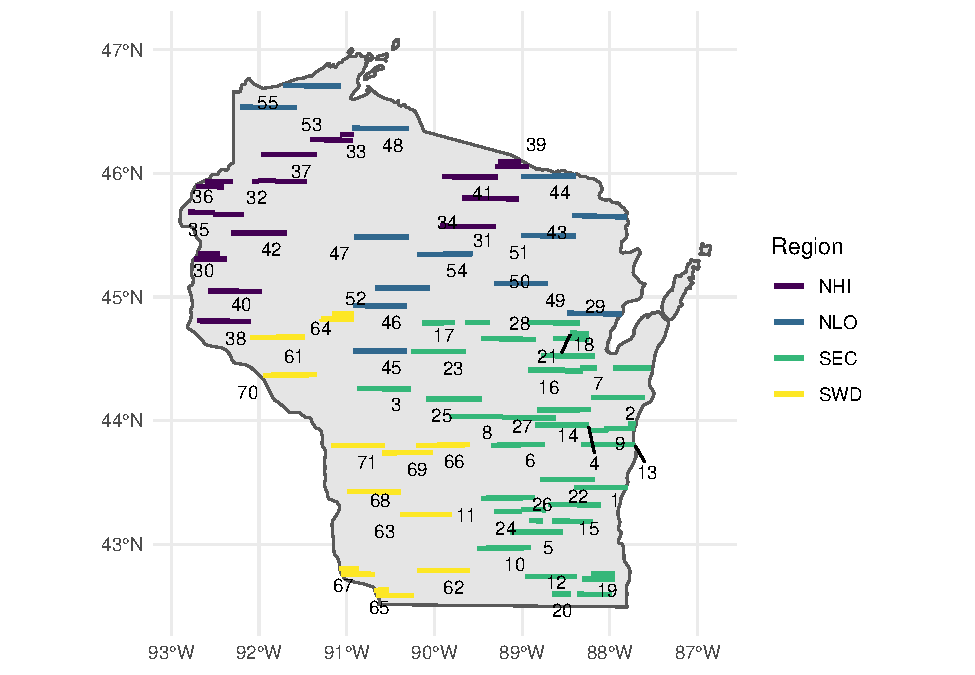
\includegraphics{/central/OAS/WATERF~1/WATERF~1/AERIAL~1/reports/2022/OAS_SP~1/figure-latex/transect_map-1.pdf}
\caption{\label{fig:transect_map}Wisconsin Waterfowl Breeding Population
Survey aerial transects (\emph{n} = 66) labeled by transect number and
survey region. The four regions surveyed are the Northern High Density
region (NHI), Northern Low Density region (NLO), Southeast Central
region (SEC), and Southwest Driftless region (SWD).}
\end{figure}

\newpage

\begin{figure}
\centering
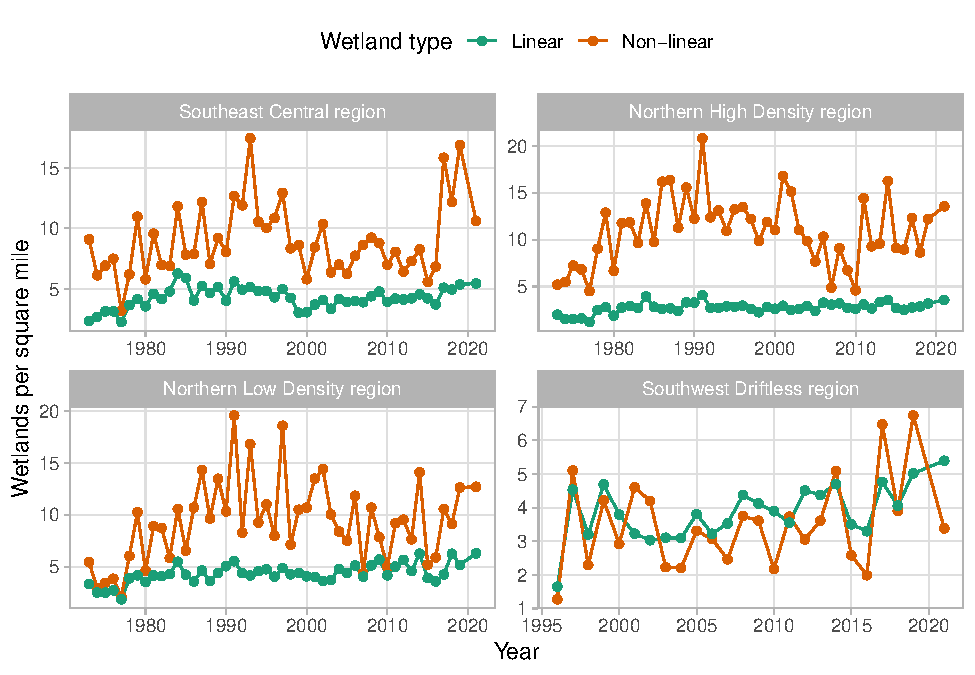
\includegraphics{/central/OAS/WATERF~1/WATERF~1/AERIAL~1/reports/2022/OAS_SP~1/figure-latex/wetland_abundance-1.pdf}
\caption{\label{fig:wetland_abundance}Annual variability in total linear
and non-linear wetlands per square mile by survey region. Note that
surveys were not conducted in 2020 due to the COVID-19 pandemic.}
\end{figure}

\newpage

\begin{figure}
\centering
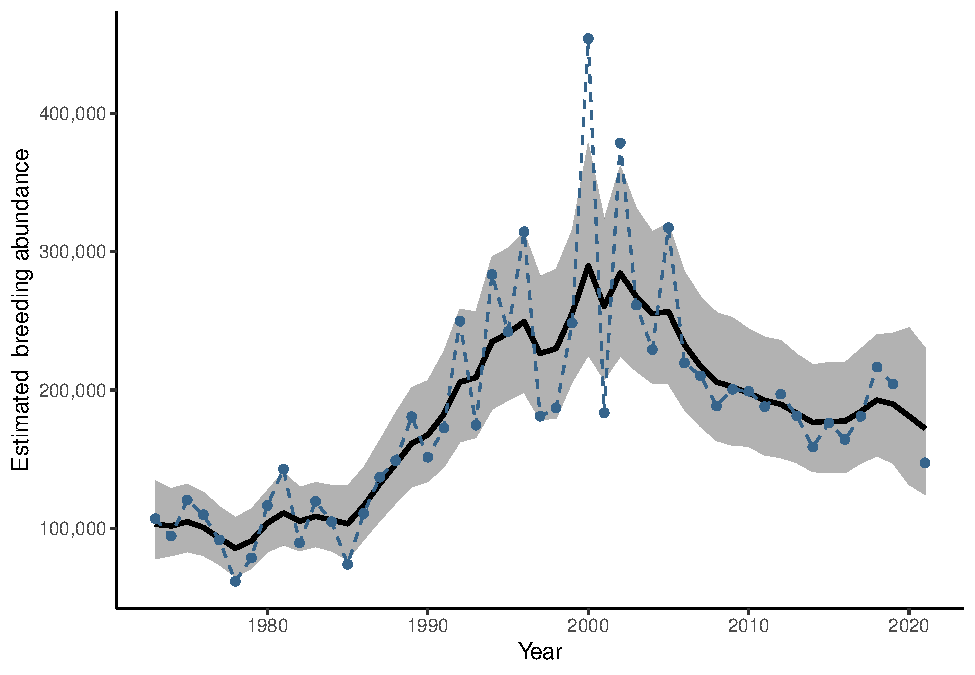
\includegraphics{/central/OAS/WATERF~1/WATERF~1/AERIAL~1/reports/2022/OAS_SP~1/figure-latex/ssm_mall-1.pdf}
\caption{\label{fig:ssm_mall}Annual statewide estimates of breeding
mallard population size in Wisconsin, 1973--2022. Black line and gray
shaded region are the mean and 95\% credible interval estimates for the
state-space population trend, and blue points and dashed line show the
annual survey counts. Note that surveys were not conducted in 2020 due
to the COVID-19 pandemic.}
\end{figure}

\newpage

\begin{figure}
\centering
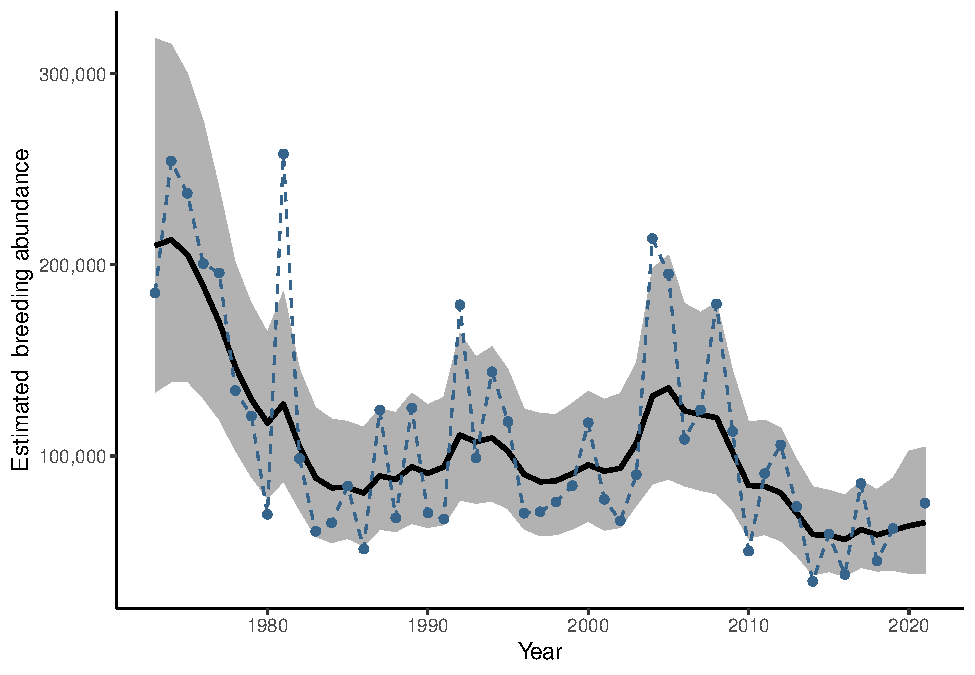
\includegraphics{/central/OAS/WATERF~1/WATERF~1/AERIAL~1/reports/2022/OAS_SP~1/figure-latex/ssm_bwte-1.pdf}
\caption{\label{fig:ssm_bwte}Annual statewide estimates of breeding
blue-winged teal abundance in Wisconsin, 1973--2022. Black line and gray
shaded region are the mean and 95\% credible interval estimates for the
state-space population trend, and blue points and dashed line show the
annual survey counts. Note that surveys were not conducted in 2020 due
to the COVID-19 pandemic.}
\end{figure}

\newpage

\begin{figure}
\centering
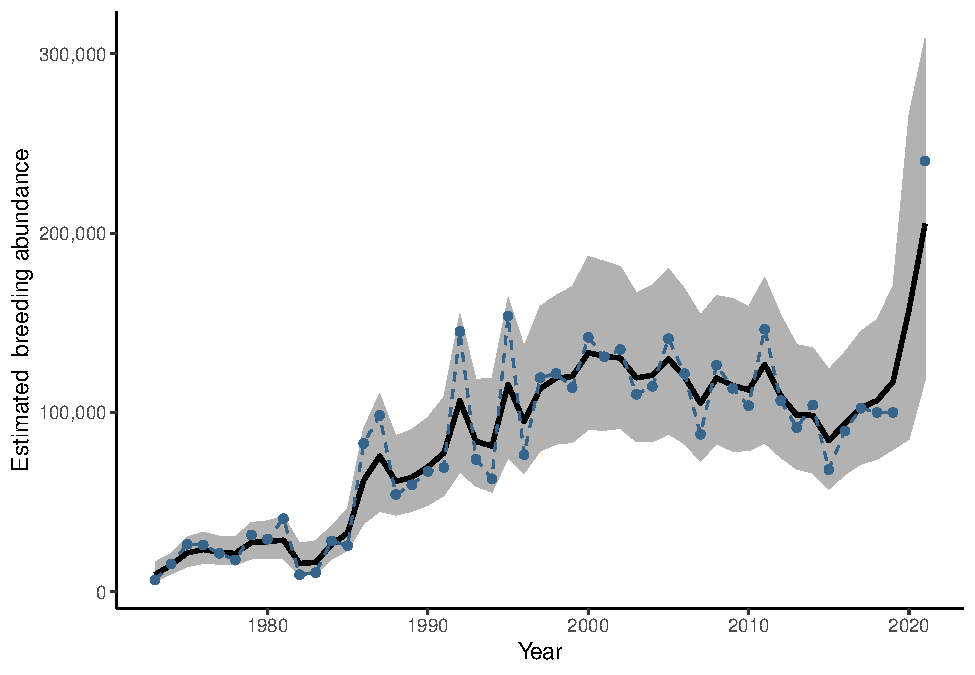
\includegraphics{/central/OAS/WATERF~1/WATERF~1/AERIAL~1/reports/2022/OAS_SP~1/figure-latex/ssm_wodu-1.pdf}
\caption{\label{fig:ssm_wodu}Annual statewide estimates of breeding wood
duck abundance in Wisconsin, 1973--2022. Black line and gray shaded
region are the mean and 95\% credible interval estimates for the
state-space population trend, and blue points and dashed line show the
annual survey counts. Note that surveys were not conducted in 2020 due
to the COVID-19 pandemic.}
\end{figure}

\newpage

\begin{figure}
\centering
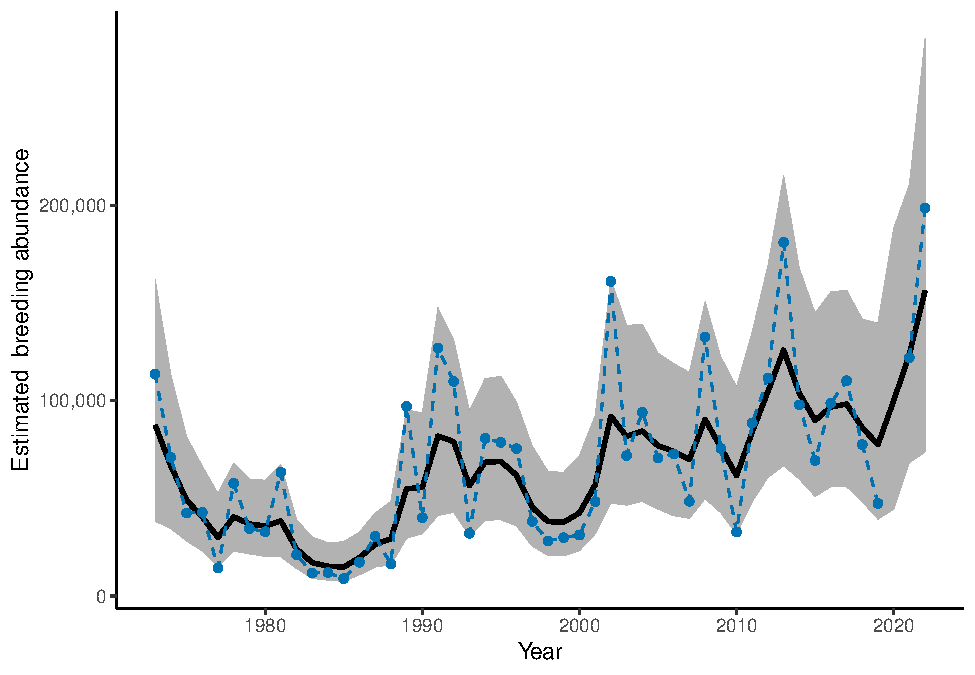
\includegraphics{/central/OAS/WATERF~1/WATERF~1/AERIAL~1/reports/2022/OAS_SP~1/figure-latex/ssm_other_ducks-1.pdf}
\caption{\label{fig:ssm_other_ducks}Annual statewide estimates of
breeding `other duck' abundance in Wisconsin, 1973--2022. Black line and
gray shaded region are the mean and 95\% credible interval estimates for
the state-space population trend, and blue points and dashed line show
the annual survey counts. Note that surveys were not conducted in 2020
due to the COVID-19 pandemic.}
\end{figure}

\newpage

\begin{figure}
\centering
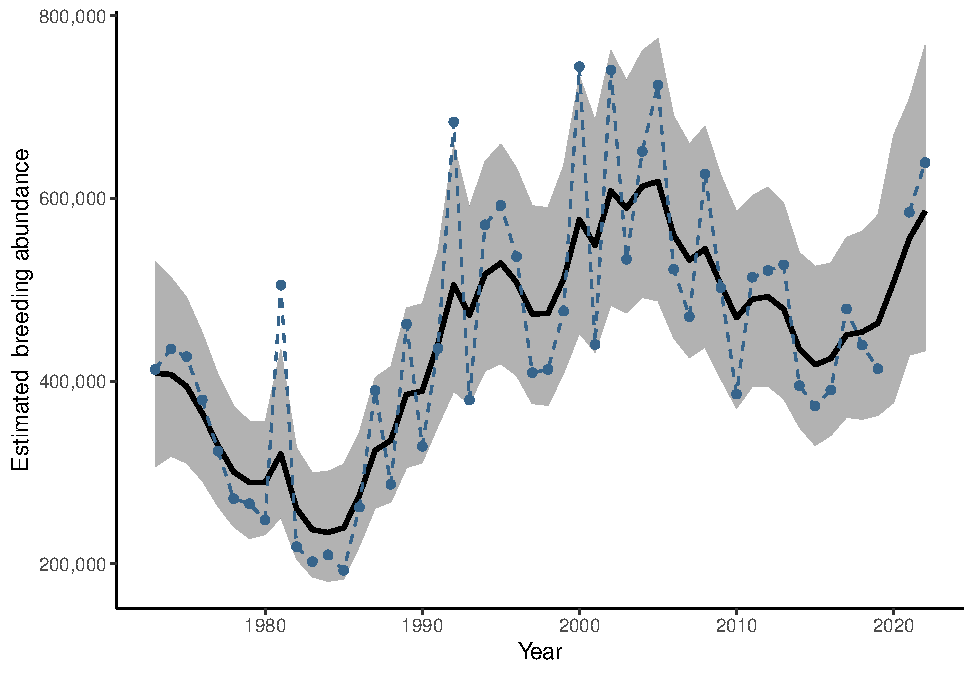
\includegraphics{/central/OAS/WATERF~1/WATERF~1/AERIAL~1/reports/2022/OAS_SP~1/figure-latex/ssm_total_ducks-1.pdf}
\caption{\label{fig:ssm_total_ducks}Annual statewide estimates of total
breeding duck abundance in Wisconsin, 1973--2022. Black line and gray
shaded region are the mean and 95\% credible interval estimates for the
state-space population trend, and blue points and dashed line show the
annual survey counts. Note that surveys were not conducted in 2020 due
to the COVID-19 pandemic.}
\end{figure}

\newpage

\begin{figure}
\centering
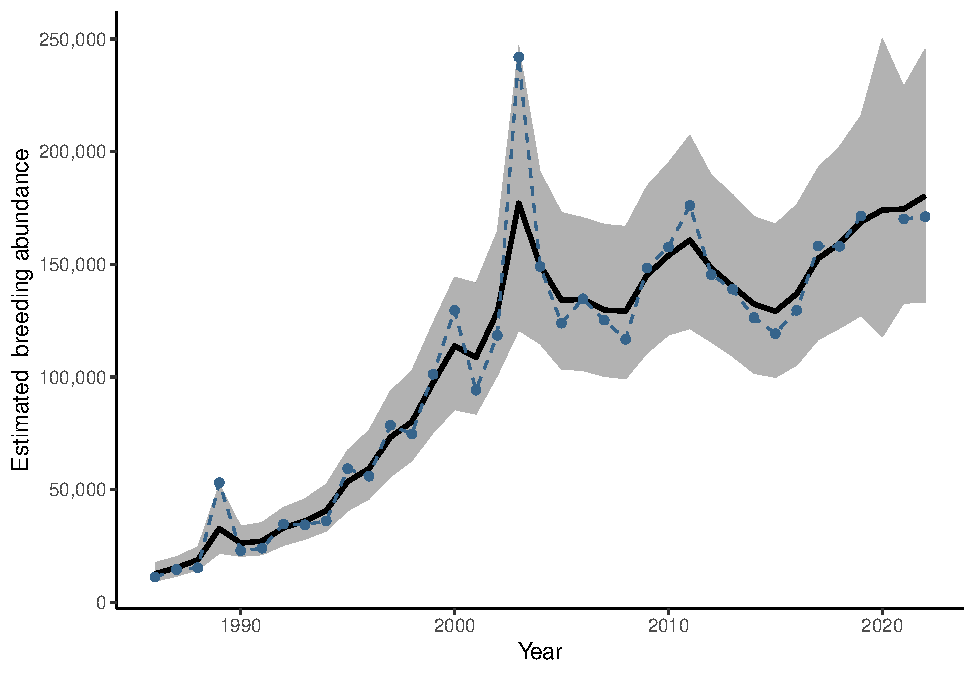
\includegraphics{/central/OAS/WATERF~1/WATERF~1/AERIAL~1/reports/2022/OAS_SP~1/figure-latex/ssm_cago-1.pdf}
\caption{\label{fig:ssm_cago}Annual statewide estimates of breeding
Canada goose abundance in Wisconsin, 1986--2022. Black line and gray
shaded region are the mean and 95\% credible interval estimates for the
state-space population trend, and blue points and dashed line show the
annual survey counts. Note that surveys were not conducted in 2020 due
to the COVID-19 pandemic.}
\end{figure}

\newpage

\begin{figure}
\centering
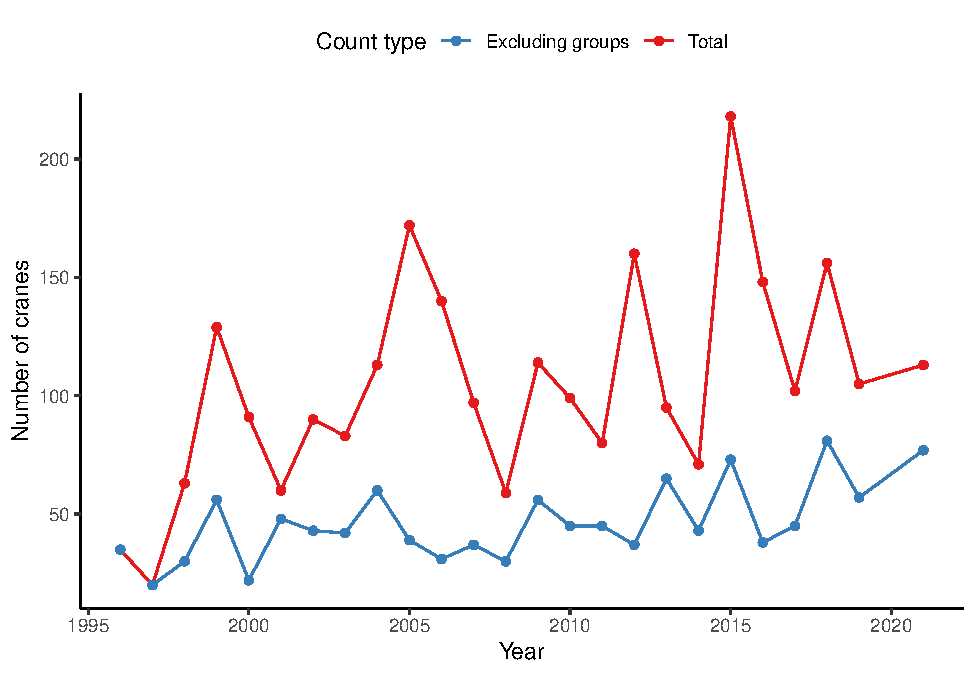
\includegraphics{/central/OAS/WATERF~1/WATERF~1/AERIAL~1/reports/2022/OAS_SP~1/figure-latex/annual_crane_counts-1.pdf}
\caption{\label{fig:annual_crane_counts}Annual counts of sandhill cranes
(raw estimates) observed from the air during the Waterfowl Breeding
Population Survey, 1996--2022. Note that surveys were not conducted in
2020 due to the COVID-19 pandemic.}
\end{figure}

\newpage

\begin{figure}
\centering
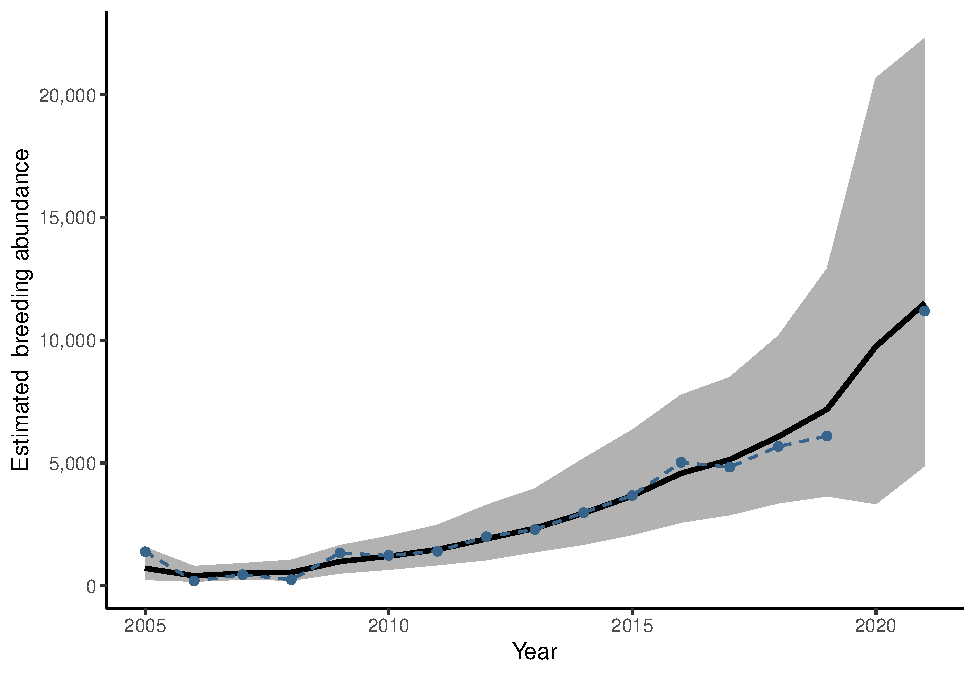
\includegraphics{/central/OAS/WATERF~1/WATERF~1/AERIAL~1/reports/2022/OAS_SP~1/figure-latex/ssm_trsw-1.pdf}
\caption{\label{fig:ssm_trsw}Annual statewide estimates of trumpeter
swan abundance in Wisconsin, 2005--2022. Black line and gray shaded
region are the mean and 95\% credible interval estimates for the
state-space population trend, and blue points and dashed line show the
annual survey counts. Note that surveys were not conducted in 2020 due
to the COVID-19 pandemic.}
\end{figure}

\end{document}
